\documentclass{article}
\usepackage[a4paper, total={7in, 9.5in}]{geometry}
\usepackage{amsmath,amsfonts,amsthm,amssymb,graphicx,float, setspace, bm}
\usepackage[utf8]{inputenc}
\usepackage{float}
\usepackage{titlesec}
\usepackage{setspace}
\usepackage{geometry}
\usepackage[style=numeric]{biblatex}
\usepackage[autostyle=true]{csquotes}
\usepackage{breqn}
\usepackage{subfig}
\usepackage[bottom]{footmisc}
\usepackage{adjustbox}
\usepackage{lipsum}
\usepackage{hyperref}
\usepackage[ruled,vlined]{algorithm2e}
\hypersetup{
    colorlinks=true,
    urlcolor=magenta
}
\usepackage[table,x11names]{xcolor}

\usepackage{xltabular}
\usepackage{multirow}
\usepackage{booktabs}




\renewcommand{\baselinestretch}{1.5} 
\setlength\parindent{0pt}
%----------------------------------------------------------------------------------------
%	START
%----------------------------------------------------------------------------------------

\newcommand{\horrule}[1]{\rule{\linewidth}{#1}}

\title{ \normalfont \normalsize 
\huge CPSC 532W - Homework 6}
\date{}
\author{Xiaoxuan Liang - 48131163}
\def\cond{\; | \;}

\begin{document}

\maketitle

\begin{enumerate}
\item Code snippets: 
\begin{figure}[!htp]
	\centering
	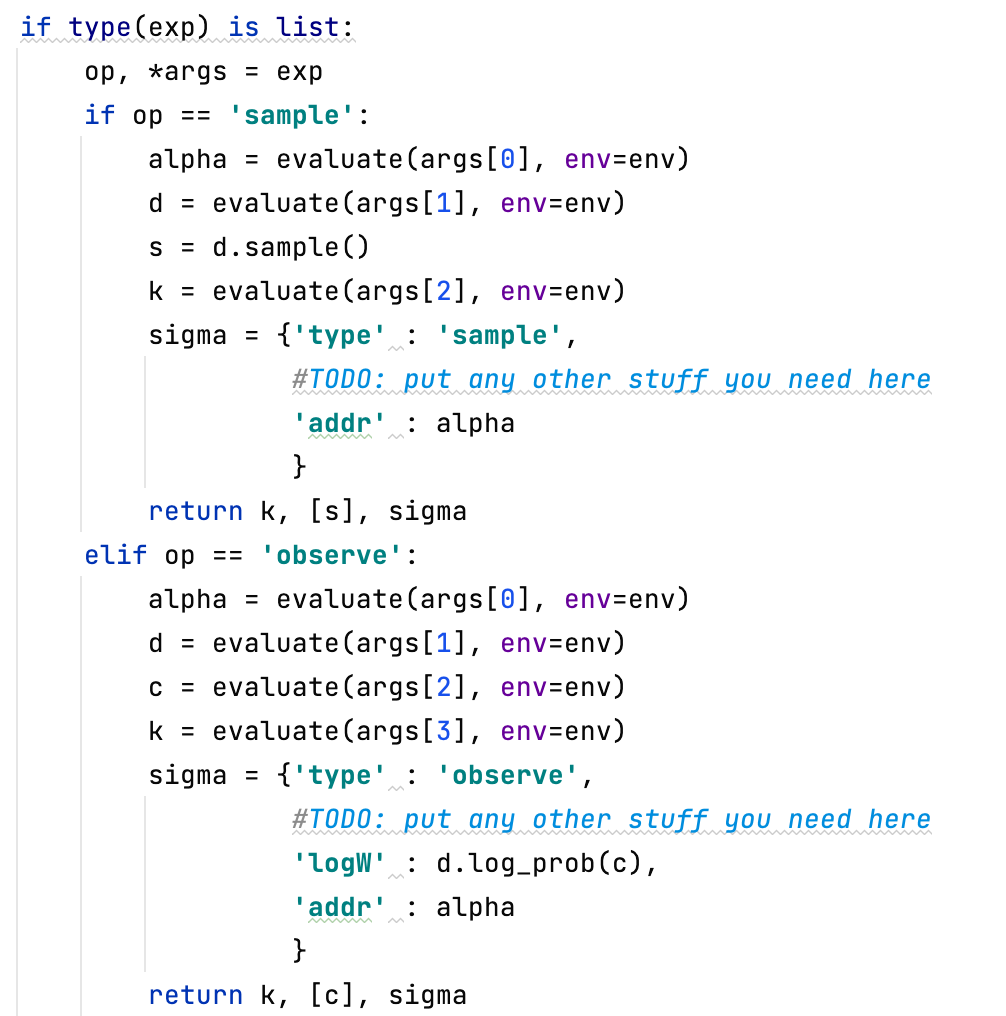
\includegraphics[scale=0.5]{../figs/code_1}
	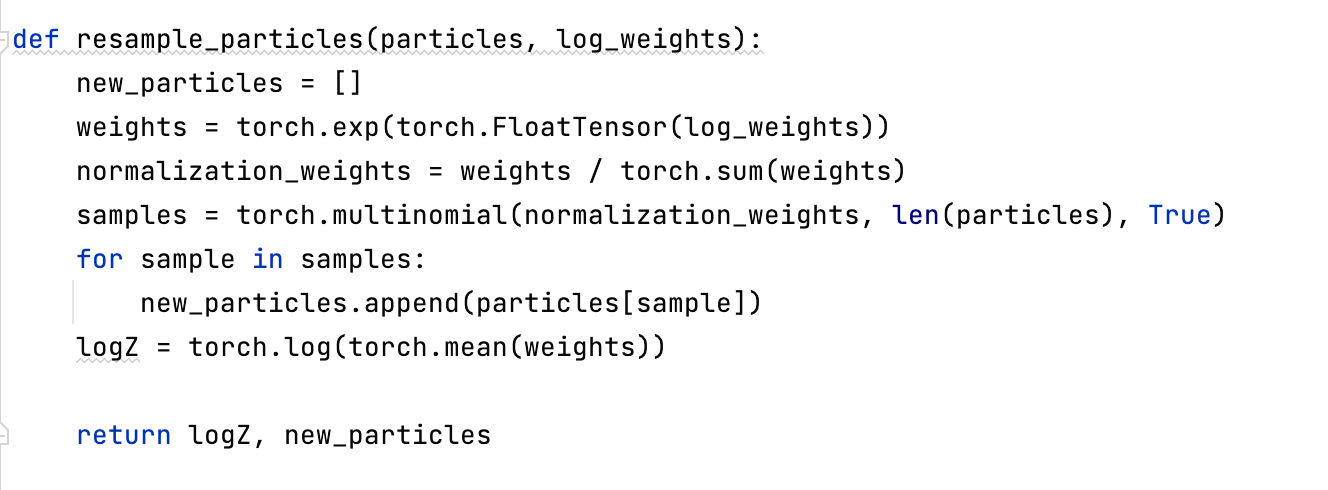
\includegraphics[scale=0.5]{../figs/code_2}
	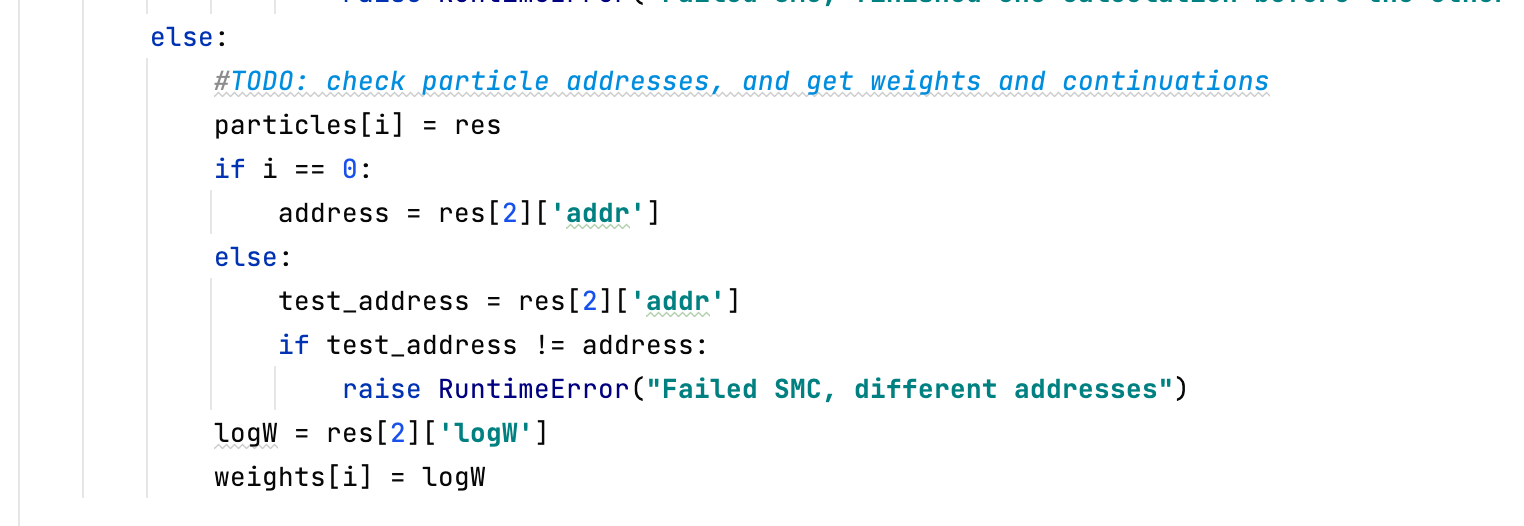
\includegraphics[scale=0.5]{../figs/code_3}
\end{figure}

\newpage
\item Program 1

\begin{figure}[!htp]
	\centering
	 \subfloat[Samples from the posterior for mu]{%
        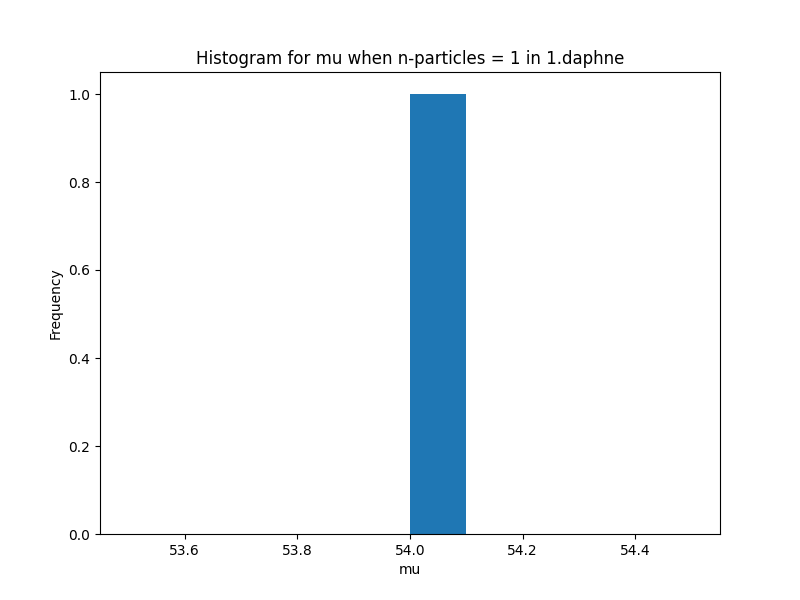
\includegraphics[width=0.5\textwidth]{../figs/1_daphne_1}%
        \label{fig:a}%
        }%
    \hfill%
    \subfloat[Samples from the posterior for mu]{%
        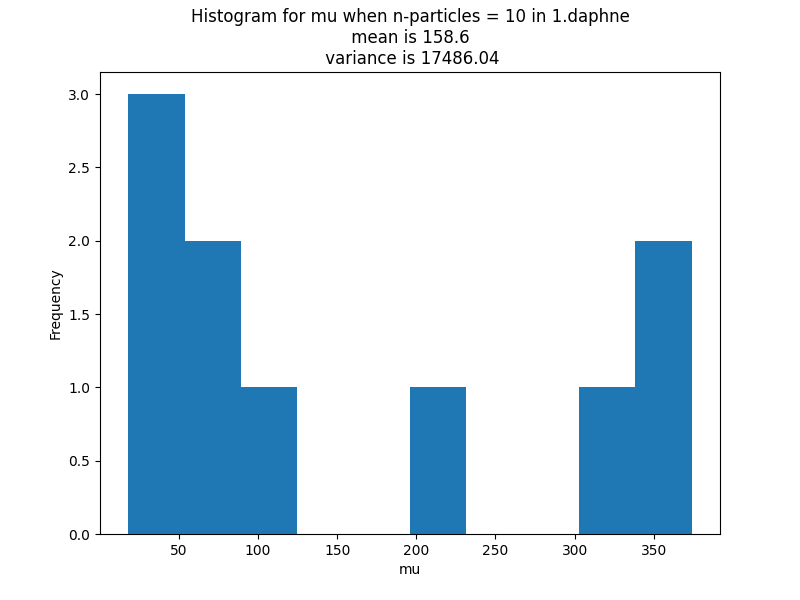
\includegraphics[width=0.5\textwidth]{../figs/1_daphne_10}%
        \label{fig:b}%
        }%
   \centering
   
   \subfloat[Samples from the posterior for mu]{%
   	  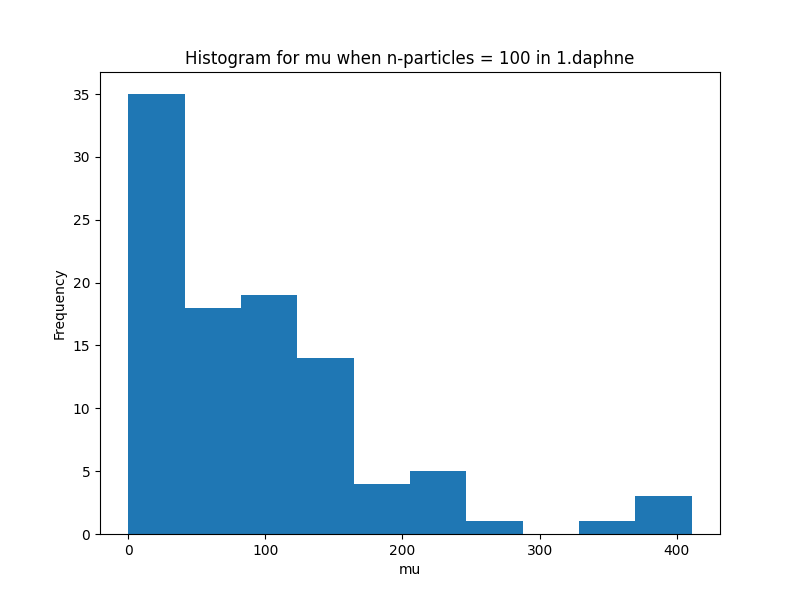
\includegraphics[width=0.5\textwidth]{../figs/1_daphne_100}%
   	  \label{fig:a}%
   	  }%
   \hfill%
	 \subfloat[Samples from the posterior for mu]{%
        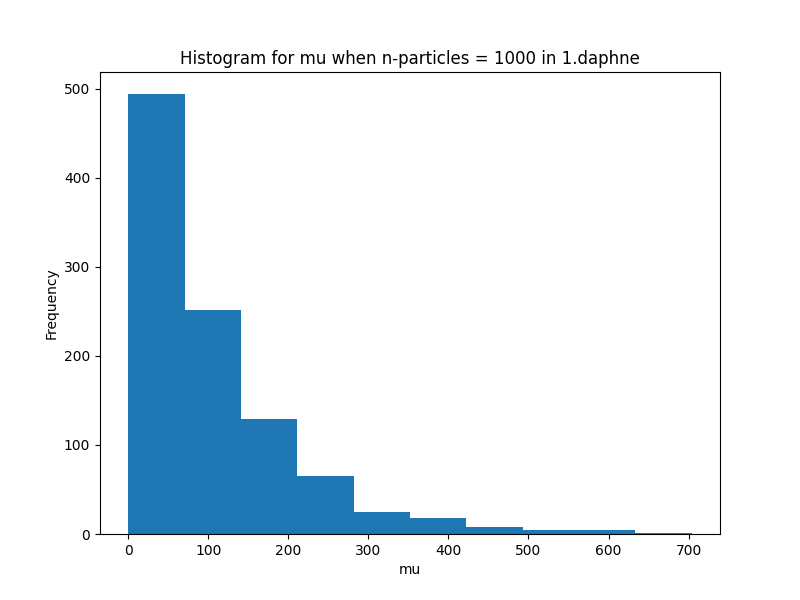
\includegraphics[width=0.5\textwidth]{../figs/1_daphne_1000}%
        \label{fig:d}%
        }%

	\centering
	 \subfloat[Samples from the posterior for mu]{%
        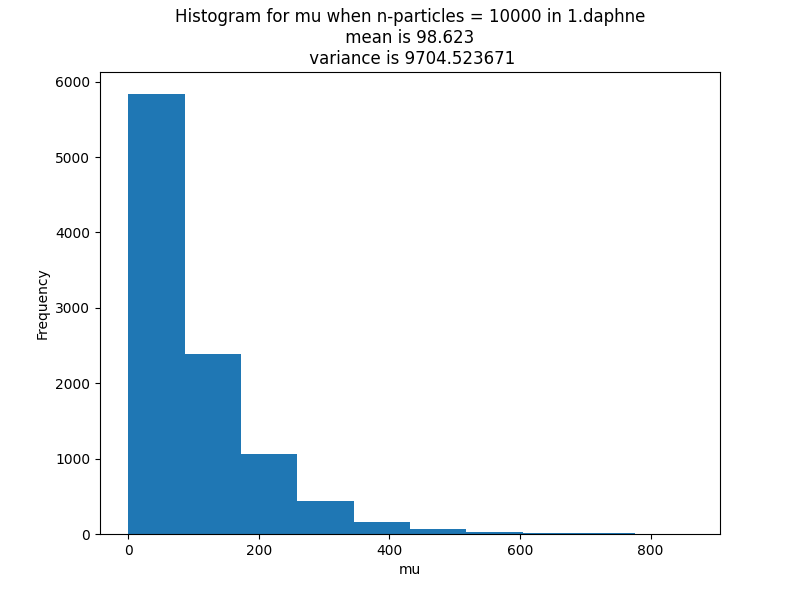
\includegraphics[width=0.5\textwidth]{../figs/1_daphne_10000}%
        \label{fig:a}%
        }%
    \hfill%
    \subfloat[Samples from the posterior for mu]{%
        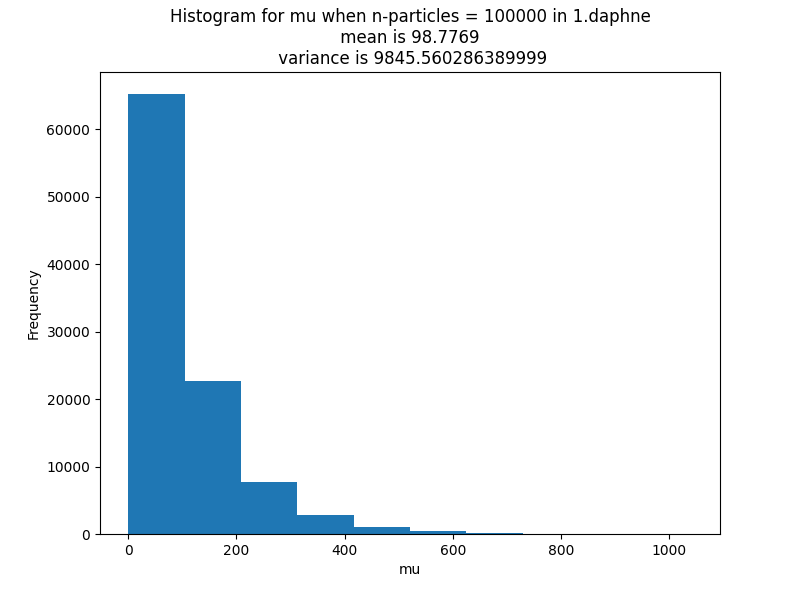
\includegraphics[width=0.5\textwidth]{../figs/1_daphne_100000}%
        \label{fig:b}%
        }%
\end{figure}

\begin{figure}
	\centering
	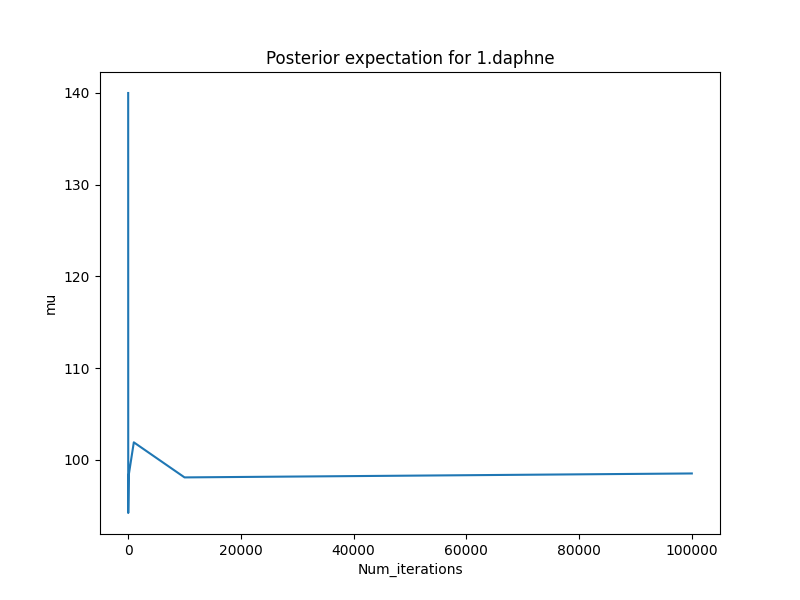
\includegraphics[scale=0.5]{../figs/1_daphne_trace_plot}
	\caption{Trace plot for posterior expectations }
\end{figure}

\newpage
\item Program 2

\begin{figure}[!htp]
	\centering
	 \subfloat[Samples from the posterior for mu]{%
        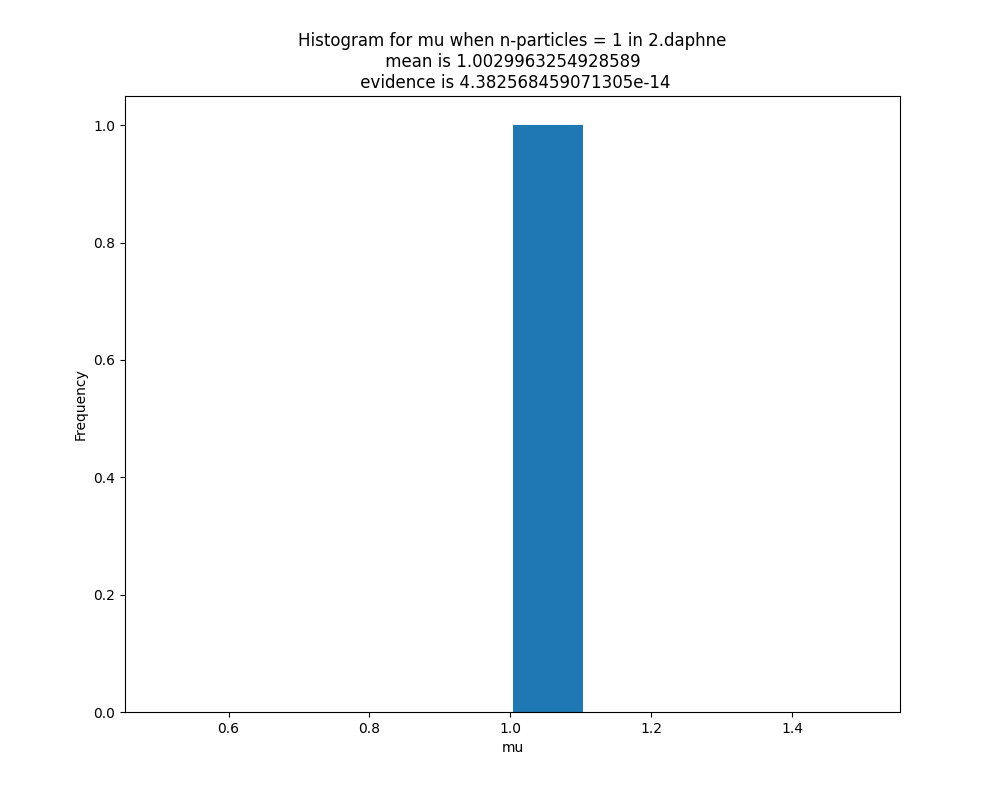
\includegraphics[width=0.5\textwidth]{../figs/2_daphne_1}%
        \label{fig:a}%
        }%
    \hfill%
    \subfloat[Samples from the posterior for mu]{%
        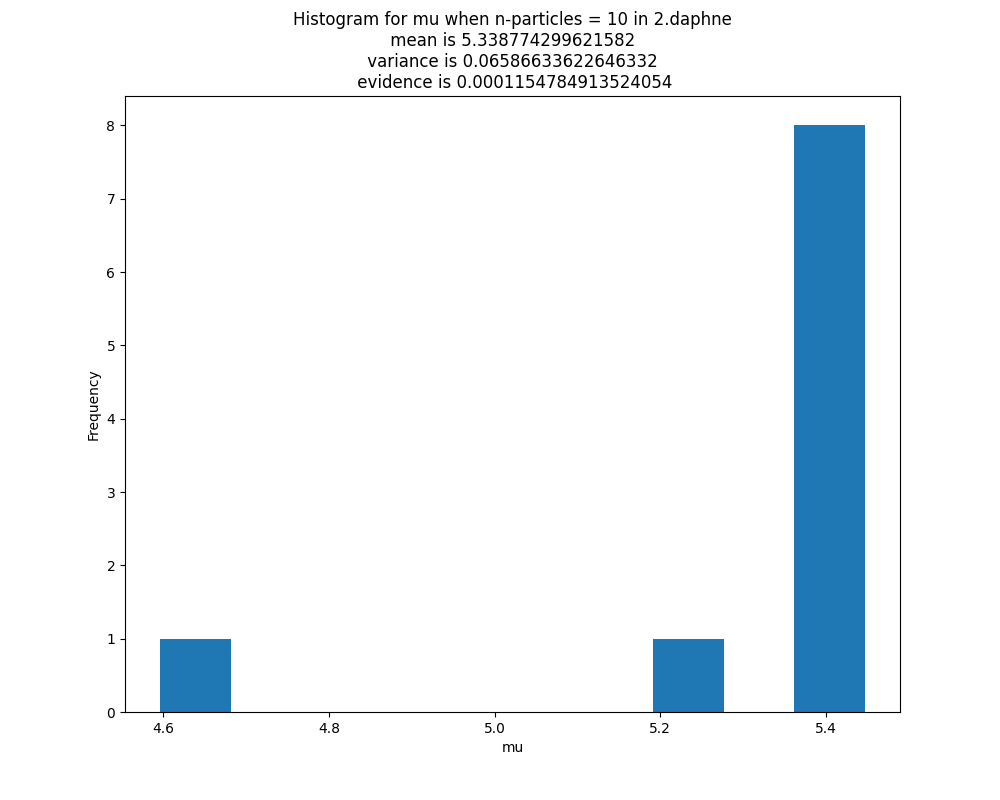
\includegraphics[width=0.5\textwidth]{../figs/2_daphne_10}%
        \label{fig:b}%
        }%
   \centering
   
   \subfloat[Samples from the posterior for mu]{%
   	  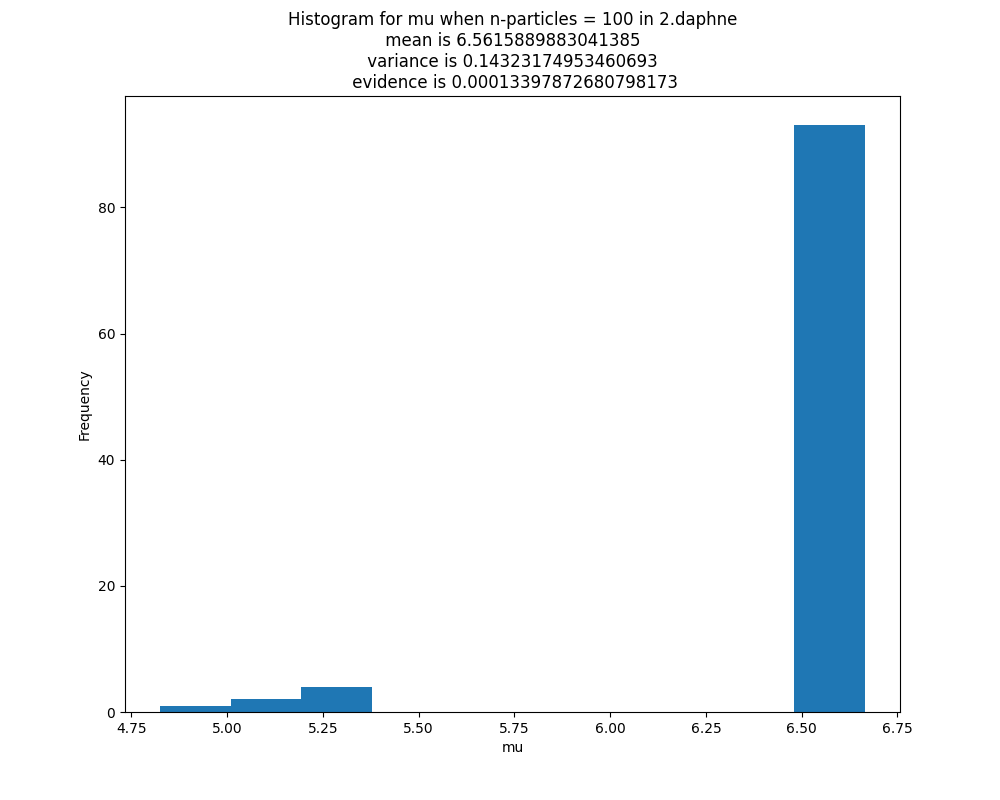
\includegraphics[width=0.5\textwidth]{../figs/2_daphne_100}%
   	  \label{fig:a}%
   	  }%
   \hfill%
	 \subfloat[Samples from the posterior for mu]{%
        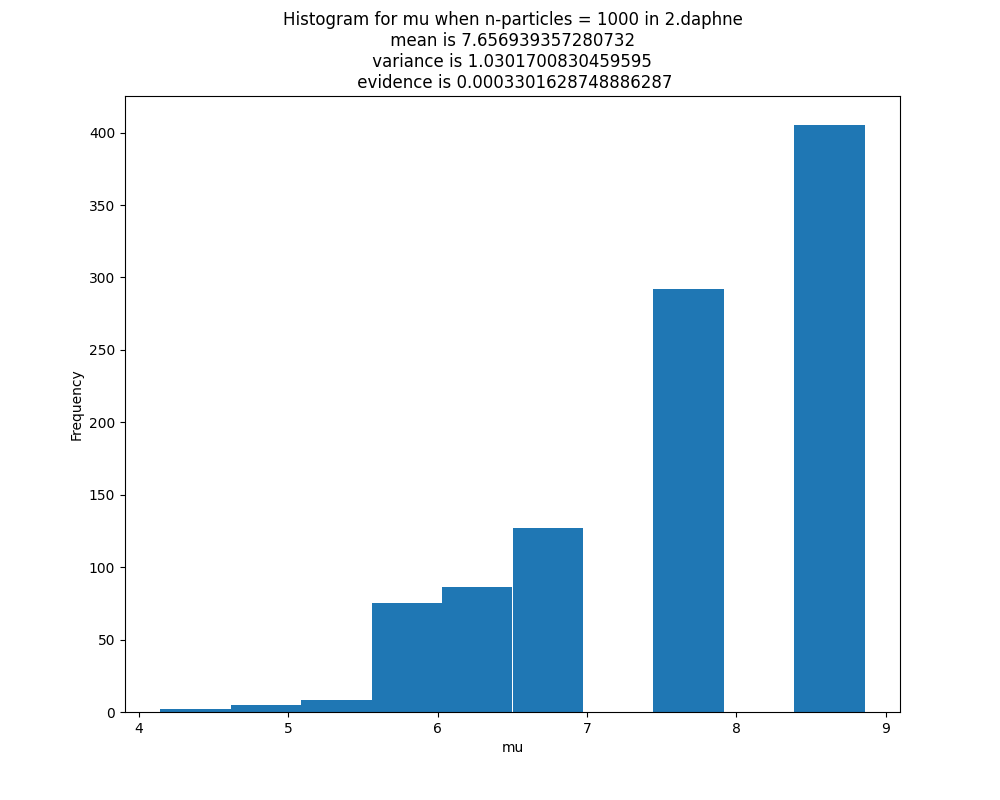
\includegraphics[width=0.5\textwidth]{../figs/2_daphne_1000}%
        \label{fig:d}%
        }%
        
	\centering
	 \subfloat[Samples from the posterior for mu]{%
        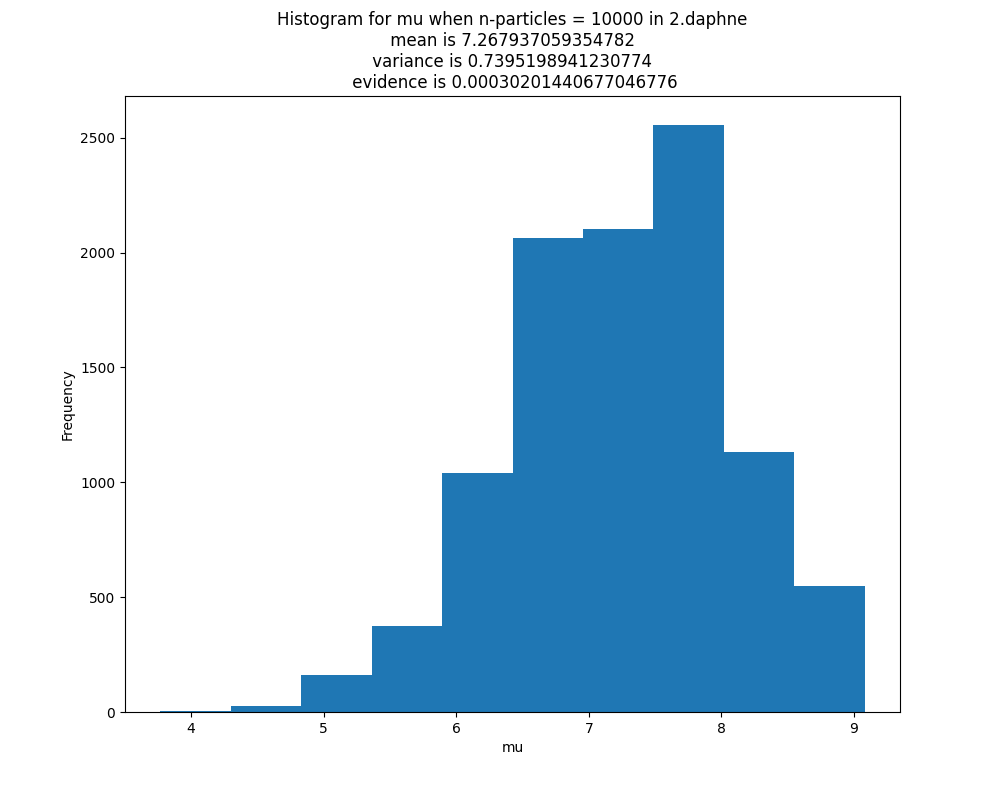
\includegraphics[width=0.5\textwidth]{../figs/2_daphne_10000}%
        \label{fig:a}%
        }%
    \hfill%
    \subfloat[Samples from the posterior for mu]{%
        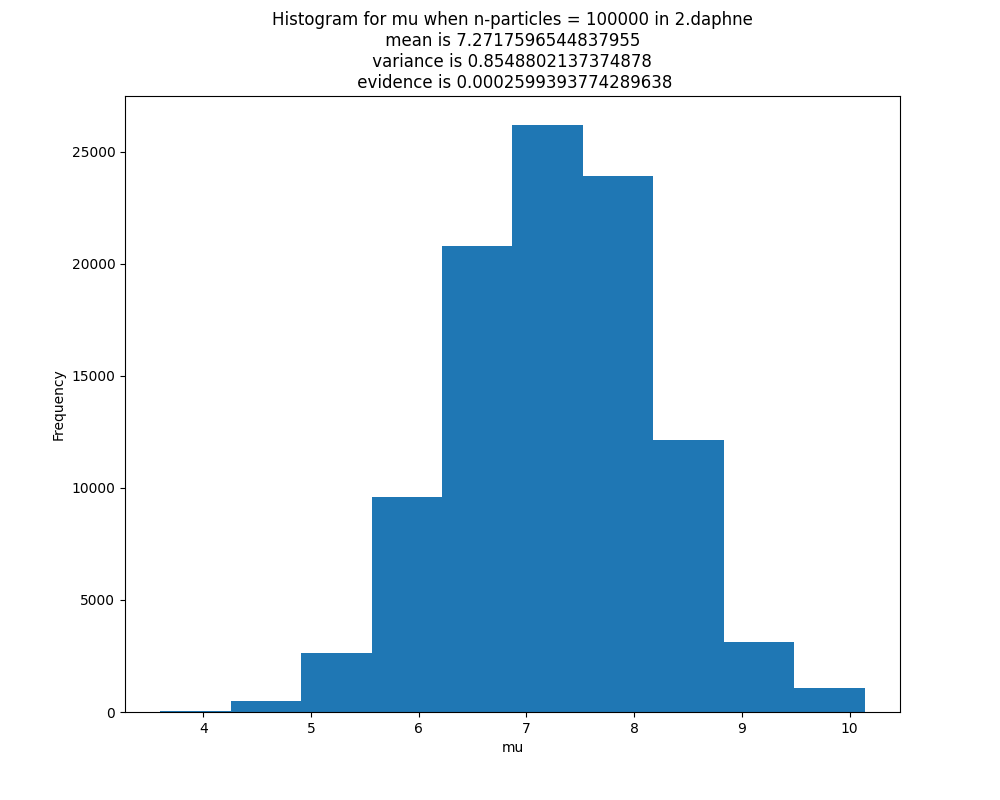
\includegraphics[width=0.5\textwidth]{../figs/2_daphne_100000}%
        \label{fig:b}%
        }%
\end{figure}

\newpage
\begin{figure}
	\centering
	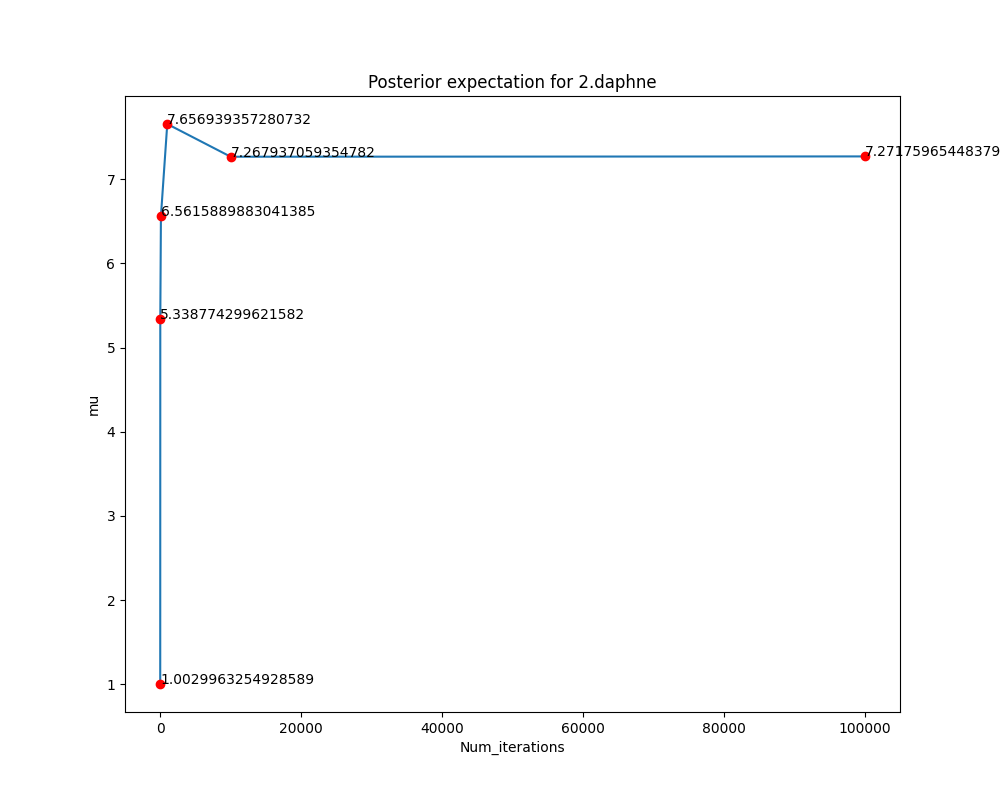
\includegraphics[scale=0.5]{../figs/2_daphne_trace_plot}
	\caption{Trace plot for posterior expectations }
\end{figure}

\begin{figure}[!ht]
	\centering
	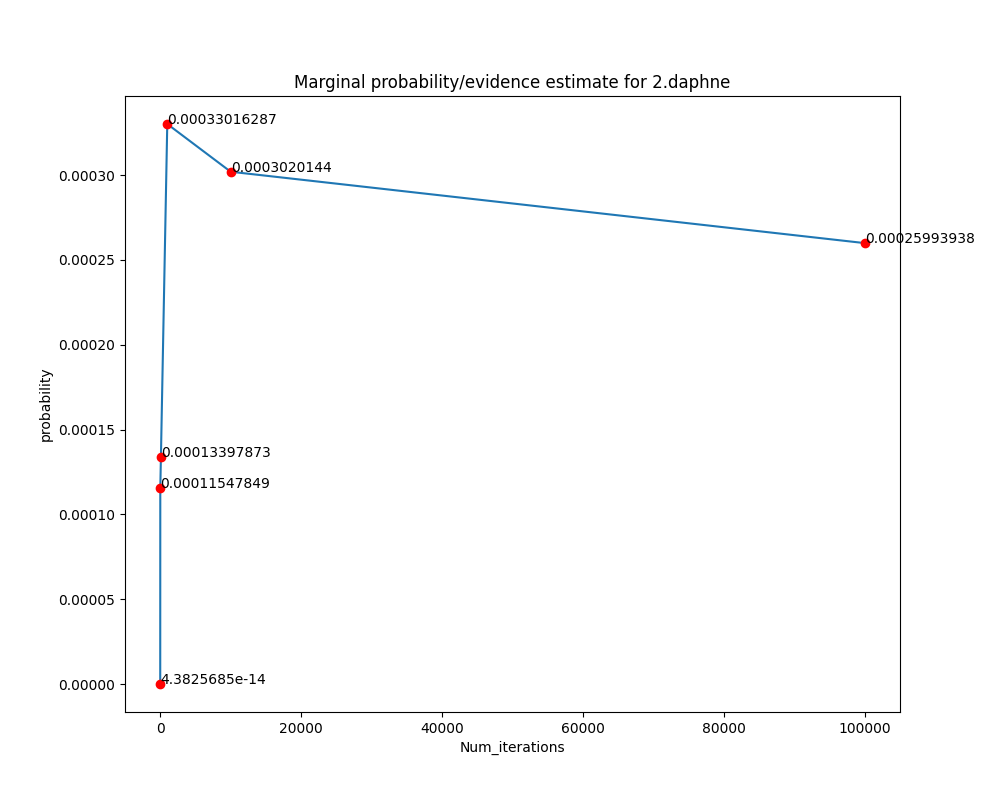
\includegraphics[scale=0.5]{../figs/2_daphne_evidence}
	\caption{evidence plot}
\end{figure}

\newpage
\item Program 3
\begin{itemize}
\item when n-particles = 1:

\begin{figure}[!htp]
	\centering
	 \subfloat[Samples from the posterior for time step]{%
        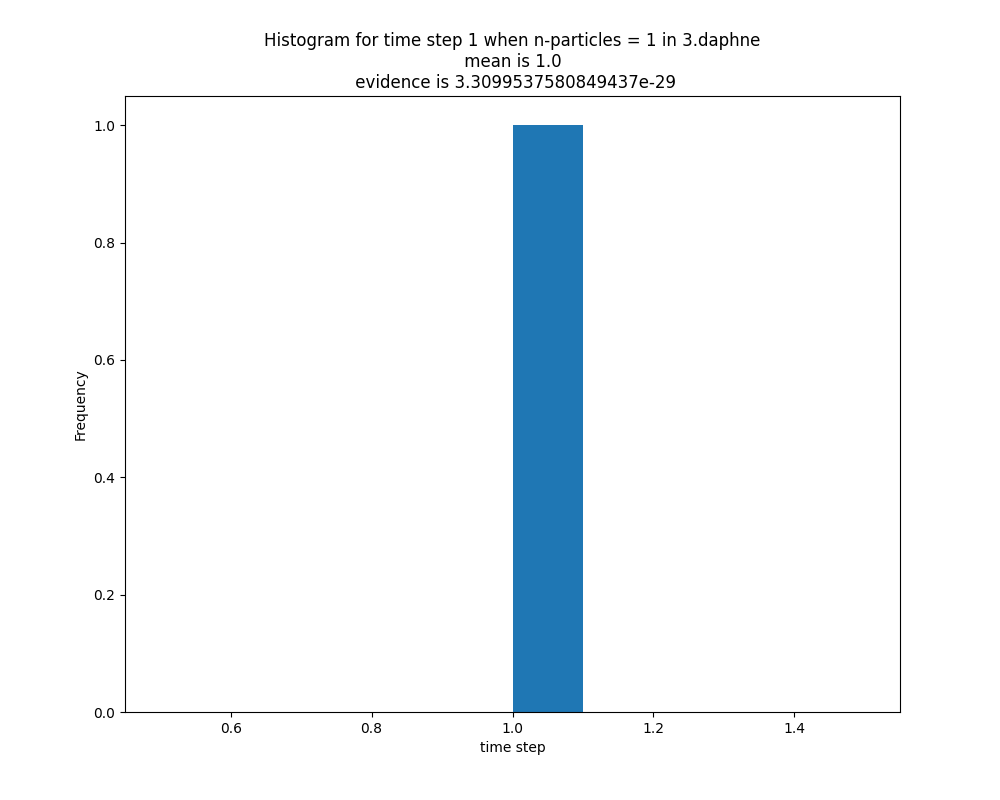
\includegraphics[width=0.3\textwidth]{../figs/3_daphne_1_1}%
        \label{fig:a}%
        }%
    \hfill%
    \subfloat[Samples from the posterior for time step]{%
        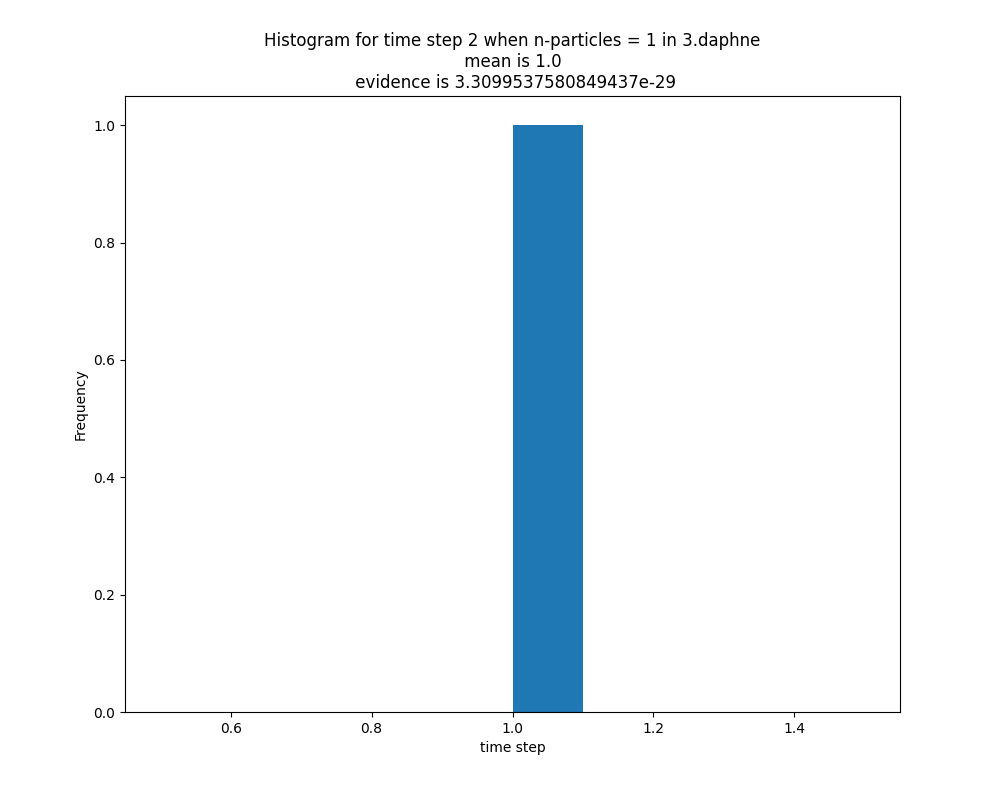
\includegraphics[width=0.3\textwidth]{../figs/3_daphne_1_2}%
        \label{fig:b}%
        }%
  \hfill
   \subfloat[Samples from the posterior for time step]{%
   	  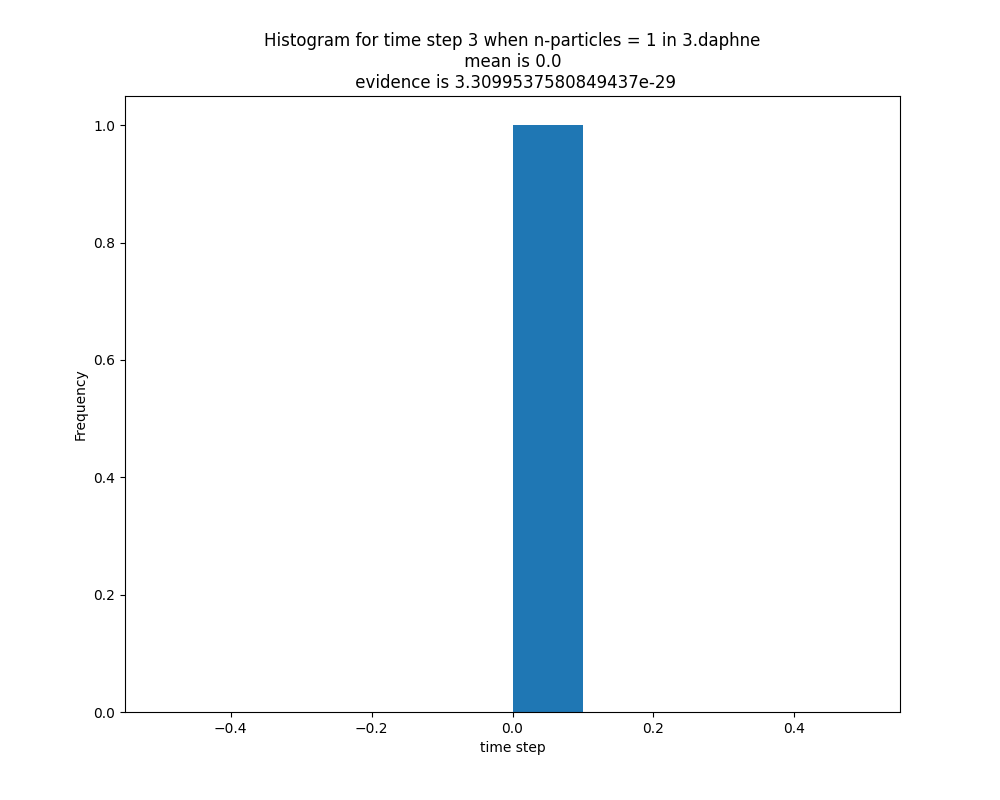
\includegraphics[width=0.3\textwidth]{../figs/3_daphne_1_3}%
   	  \label{fig:a}%
   	  }%
   	  
   \centering
	 \subfloat[Samples from the posterior for time step]{%
        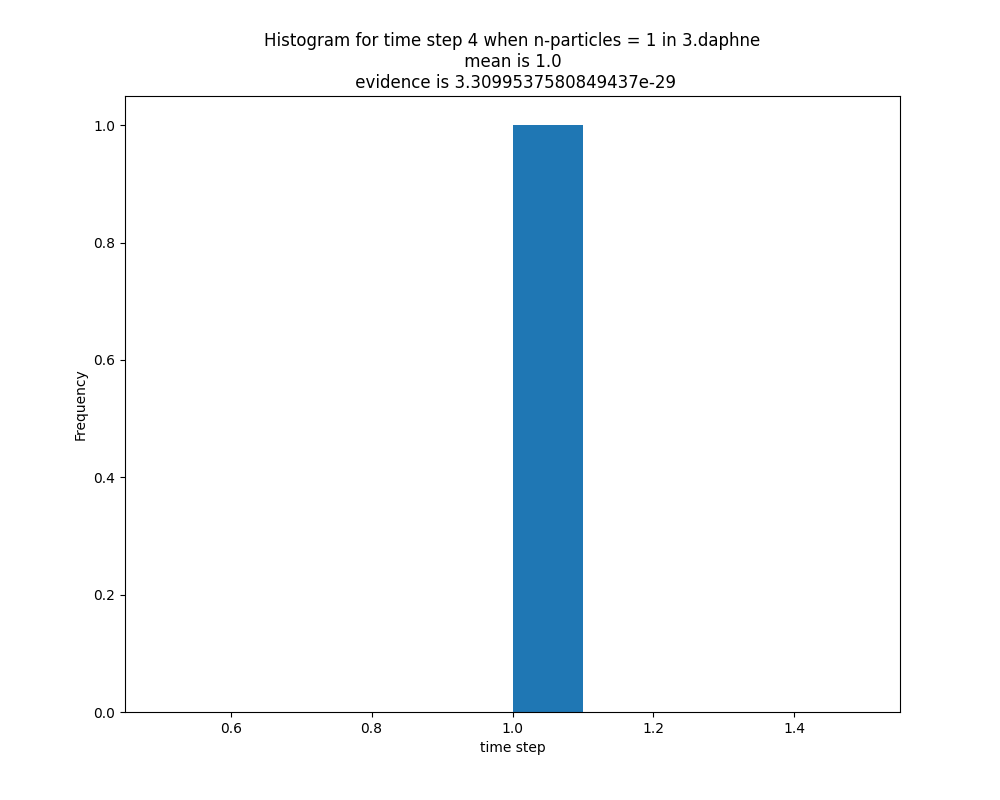
\includegraphics[width=0.3\textwidth]{../figs/3_daphne_1_4}%
        \label{fig:d}%
        }%       
	\hfill
	 \subfloat[Samples from the posterior for time step]{%
        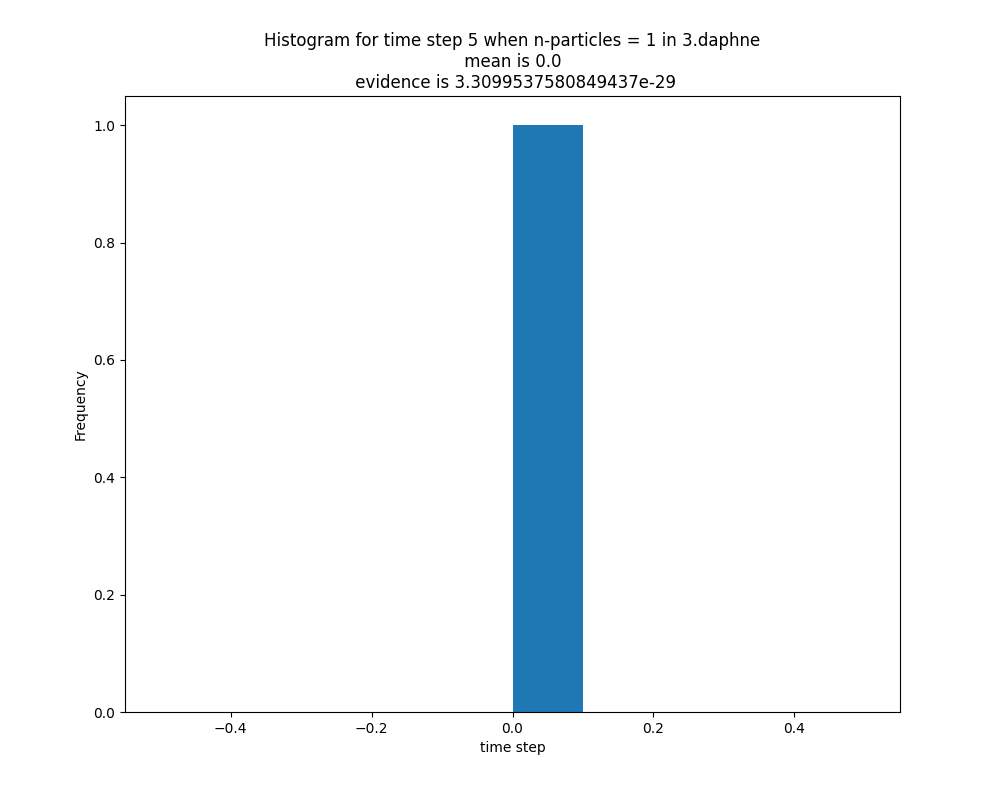
\includegraphics[width=0.3\textwidth]{../figs/3_daphne_1_5}%
        \label{fig:a}%
        }%
    \hfill%
    \subfloat[Samples from the posterior for time step]{%
        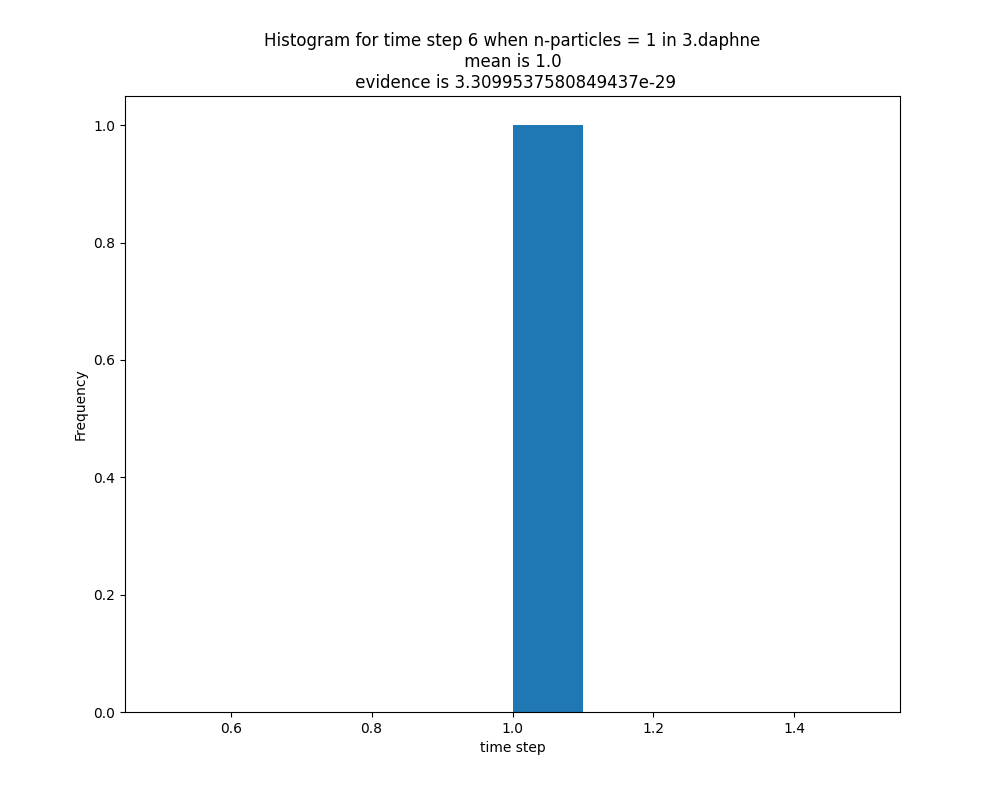
\includegraphics[width=0.3\textwidth]{../figs/3_daphne_1_6}%
        \label{fig:b}%
        }%
        
   \centering
	 \subfloat[Samples from the posterior for time step]{%
        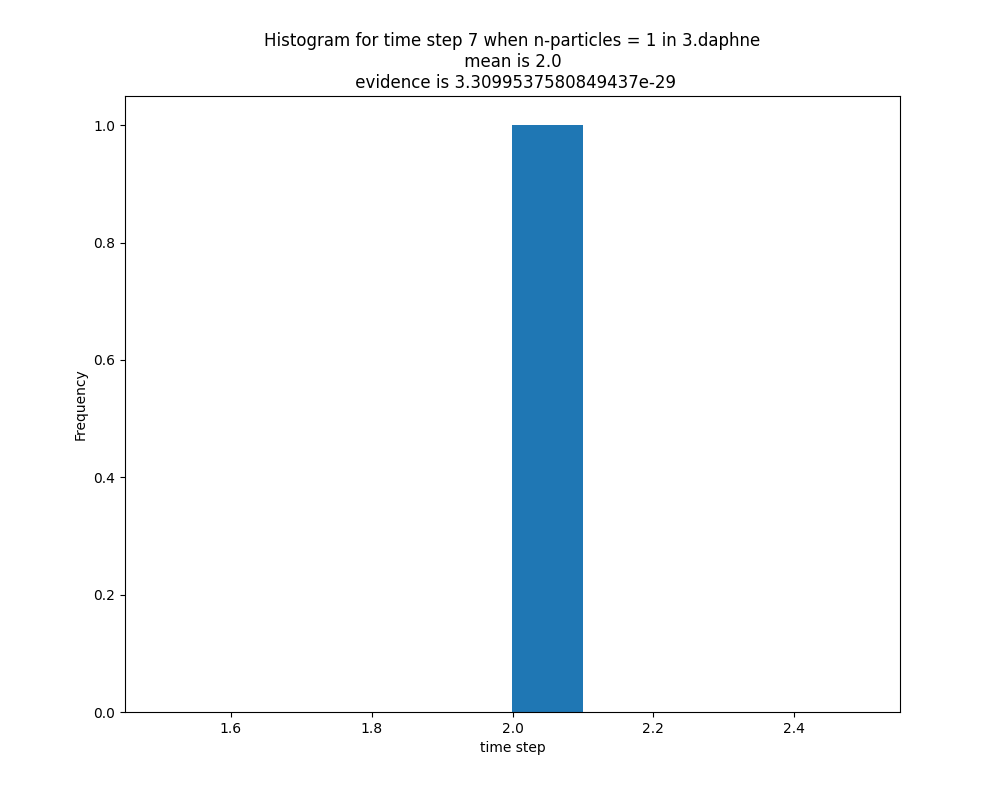
\includegraphics[width=0.3\textwidth]{../figs/3_daphne_1_7}%
        \label{fig:a}%
        }%
    \hfill%
    \subfloat[Samples from the posterior for time step]{%
        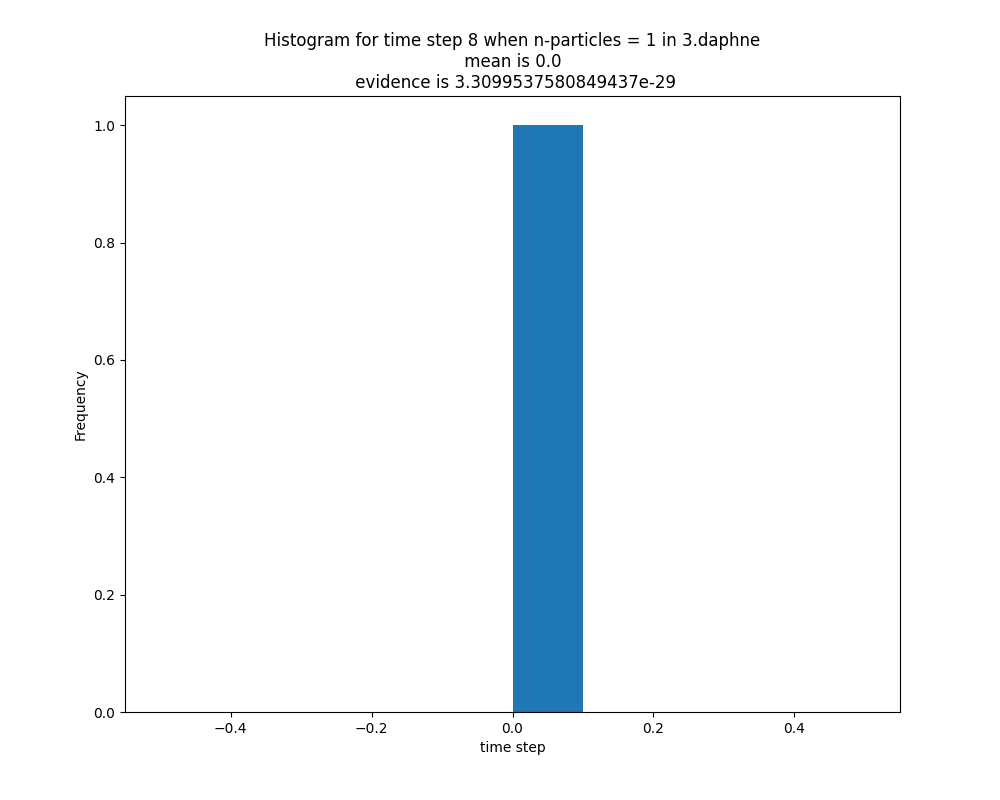
\includegraphics[width=0.3\textwidth]{../figs/3_daphne_1_8}%
        \label{fig:b}%
        }%
  \hfill
   \subfloat[Samples from the posterior for time step]{%
   	  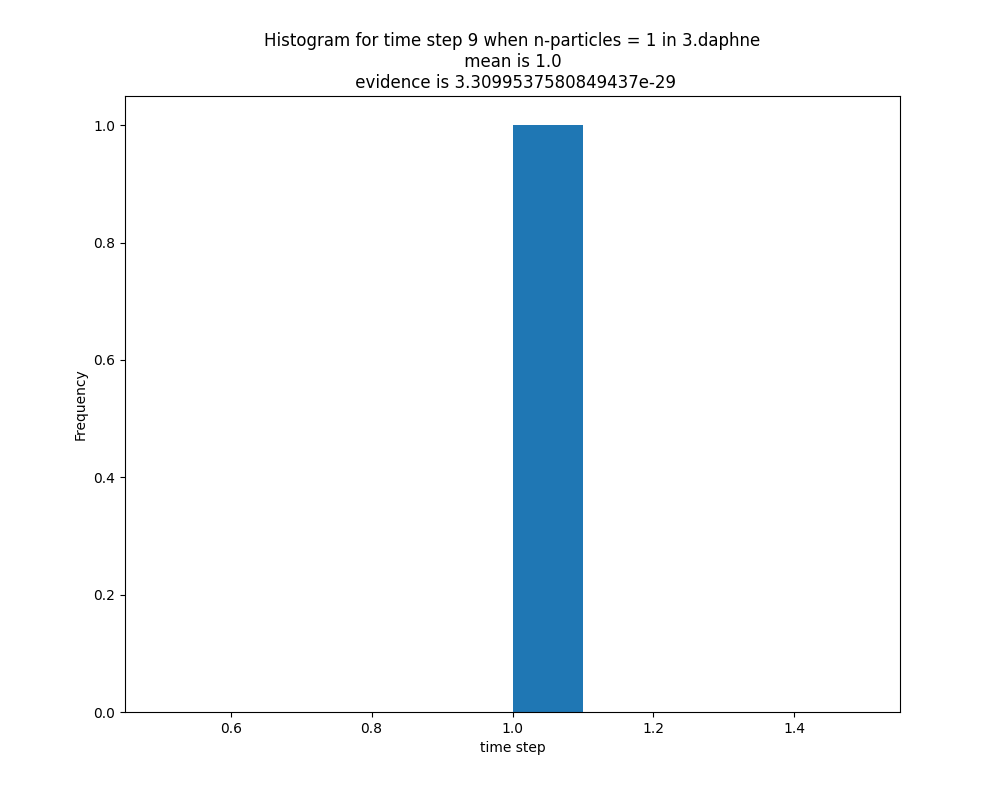
\includegraphics[width=0.3\textwidth]{../figs/3_daphne_1_9}%
   	  \label{fig:a}%
   	  }%
   	  
   \centering
	 \subfloat[Samples from the posterior for time step]{%
        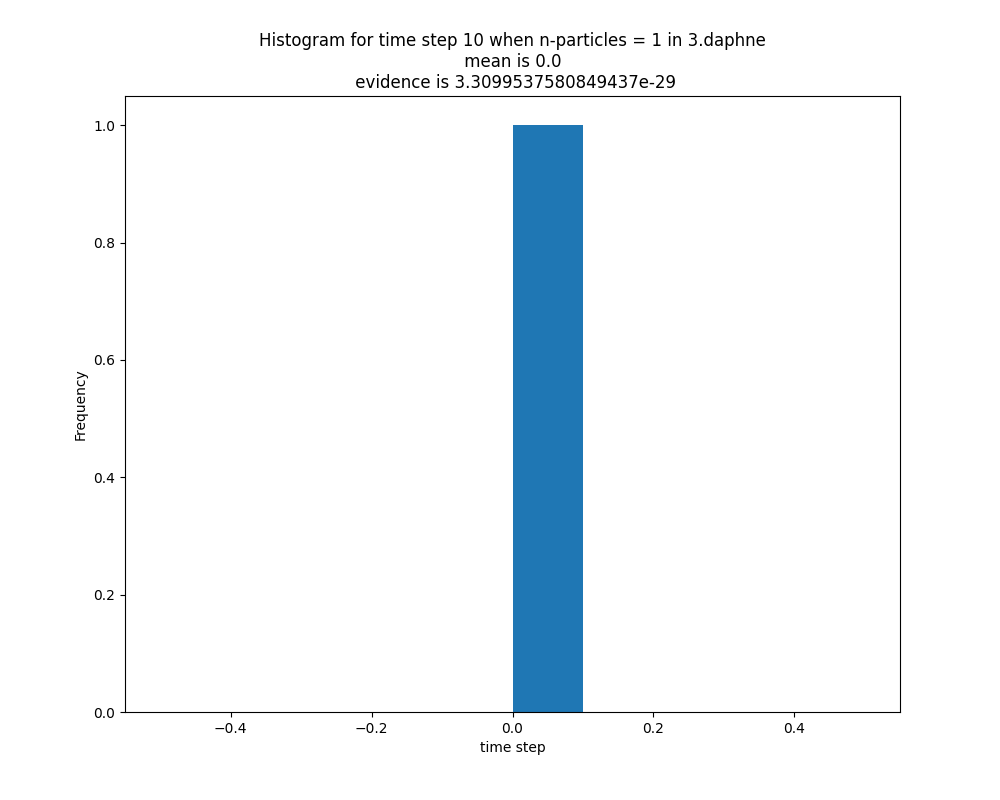
\includegraphics[width=0.3\textwidth]{../figs/3_daphne_1_10}%
        \label{fig:d}%
        }%       
	\hfill
	 \subfloat[Samples from the posterior for time step]{%
        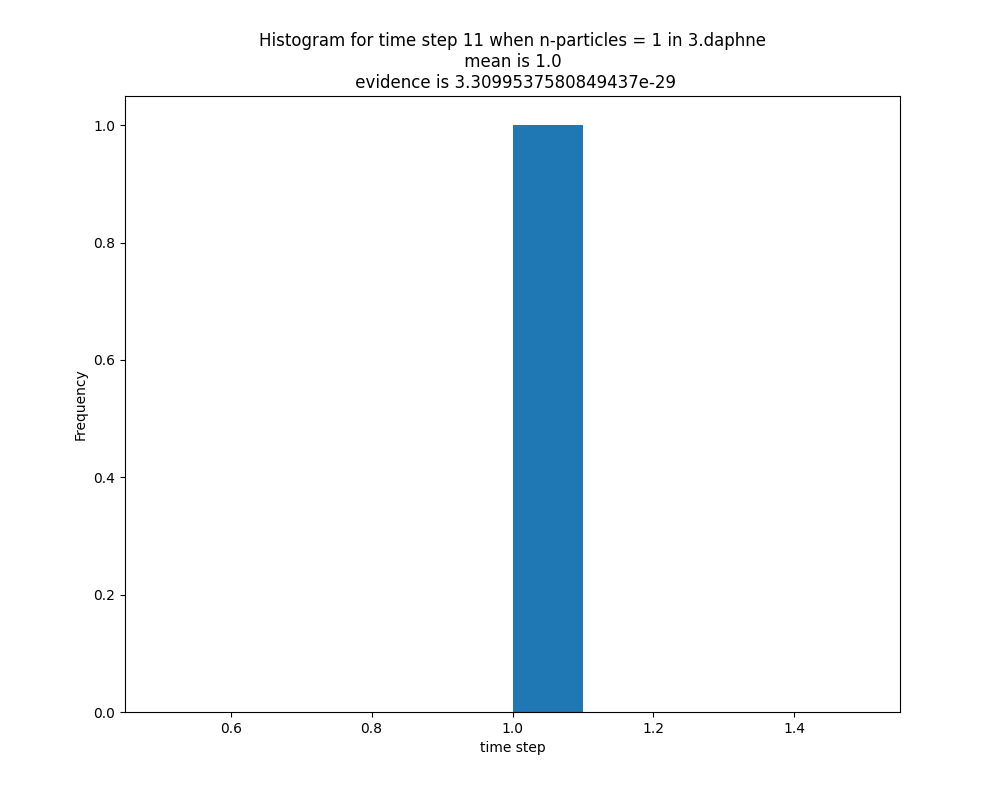
\includegraphics[width=0.3\textwidth]{../figs/3_daphne_1_11}%
        \label{fig:a}%
        }%
    \hfill%
    \subfloat[Samples from the posterior for time step]{%
        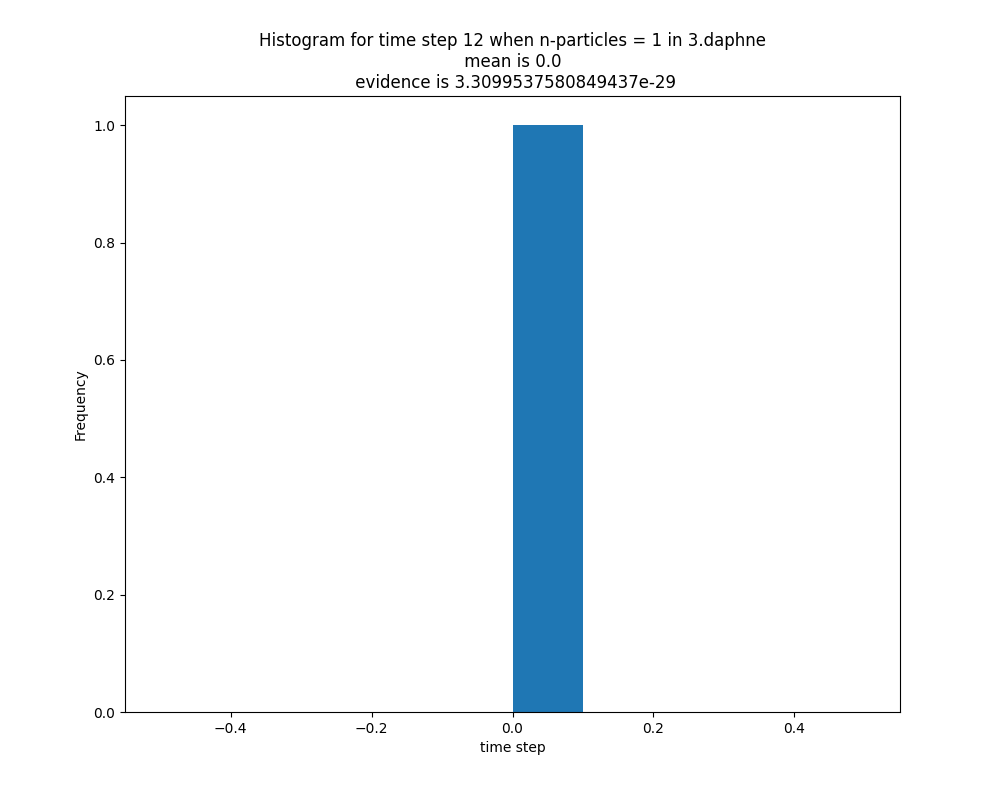
\includegraphics[width=0.3\textwidth]{../figs/3_daphne_1_12}%
        \label{fig:b}%
        }%
\end{figure}

\begin{figure}[!htp]
	\centering
	 \subfloat[Samples from the posterior for time step]{%
        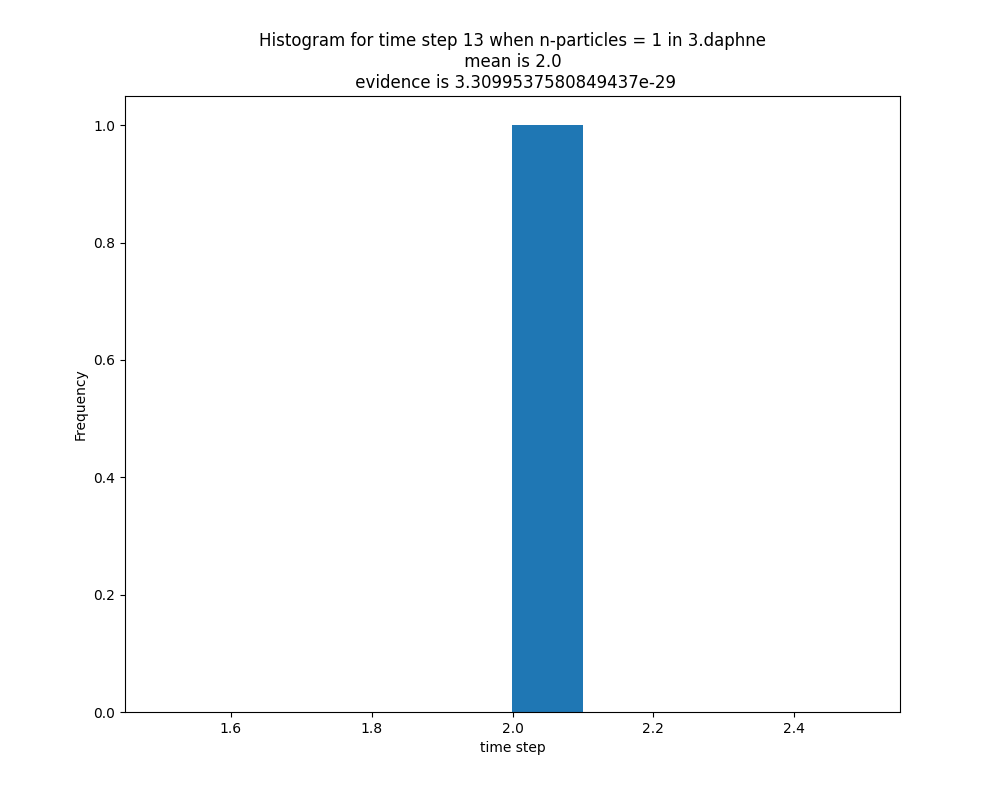
\includegraphics[width=0.3\textwidth]{../figs/3_daphne_1_13}%
        \label{fig:a}%
        }%
    \hfill%
    \subfloat[Samples from the posterior for time step]{%
        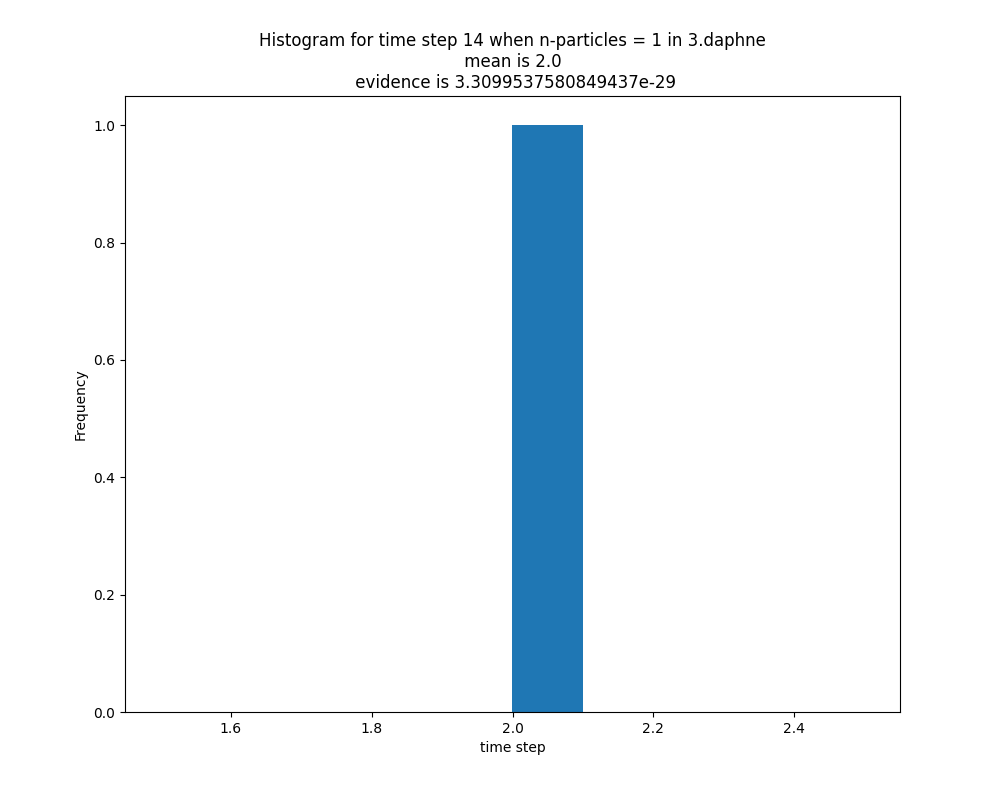
\includegraphics[width=0.3\textwidth]{../figs/3_daphne_1_14}%
        \label{fig:b}%
        }%
  \hfill
   \subfloat[Samples from the posterior for time step]{%
   	  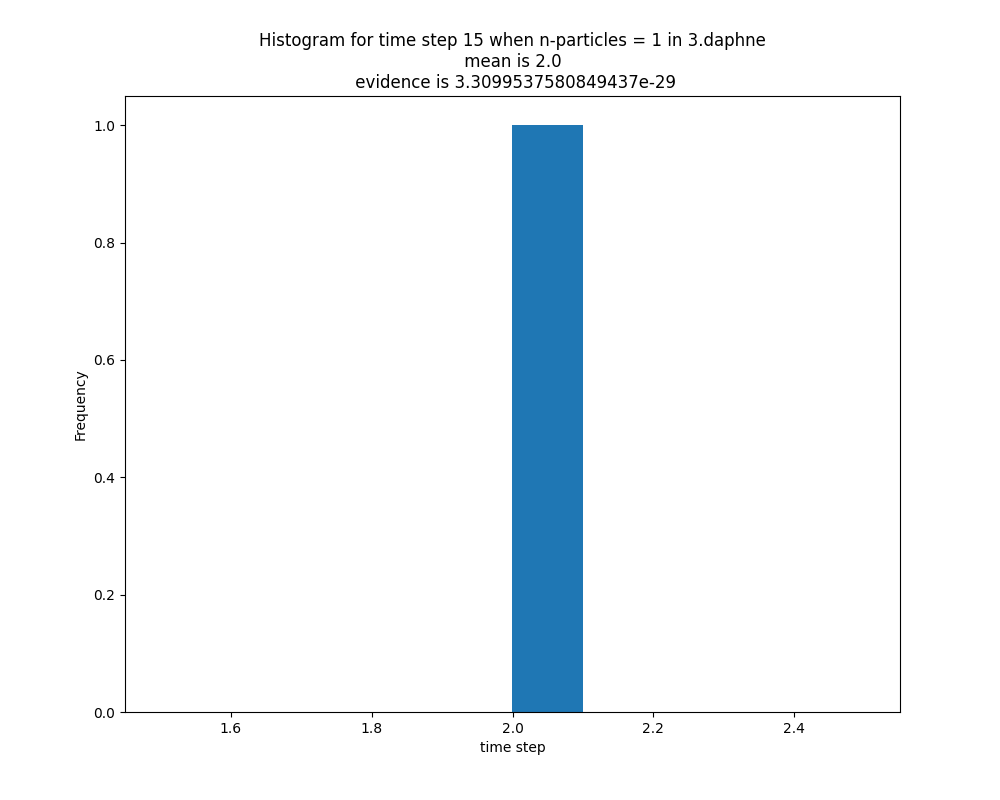
\includegraphics[width=0.3\textwidth]{../figs/3_daphne_1_15}%
   	  \label{fig:a}%
   	  }%
   	  
   \centering
	 \subfloat[Samples from the posterior for time step]{%
        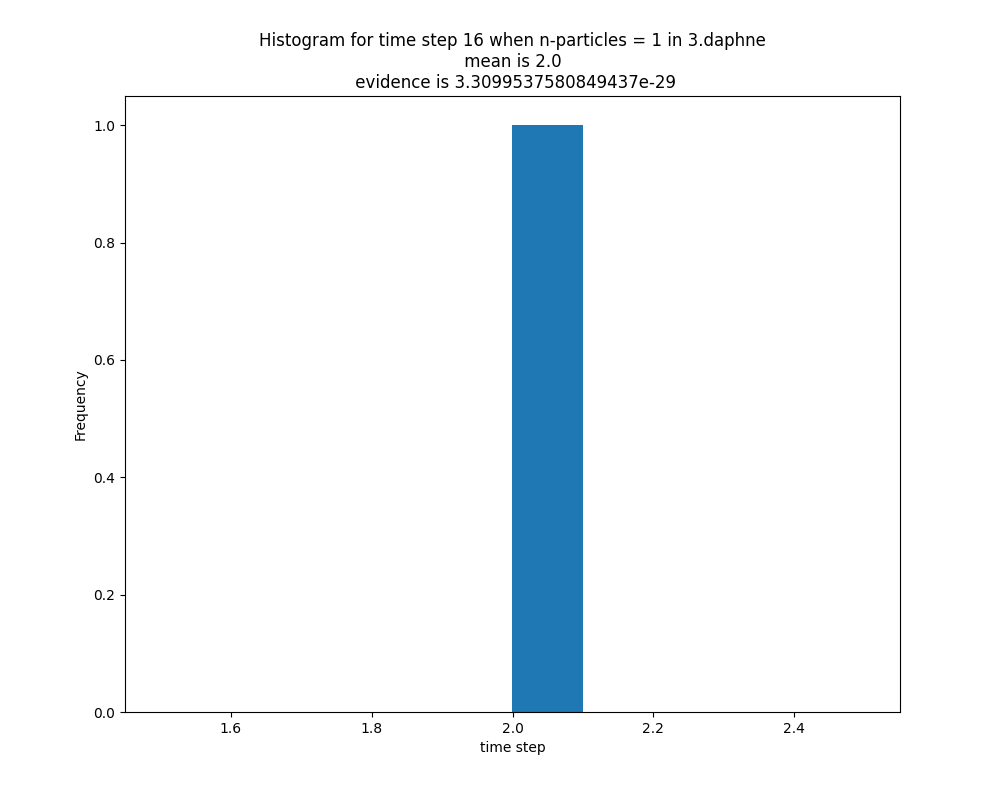
\includegraphics[width=0.3\textwidth]{../figs/3_daphne_1_16}%
        \label{fig:a}%
        }%
    \hfill%
    \subfloat[Samples from the posterior for time step]{%
        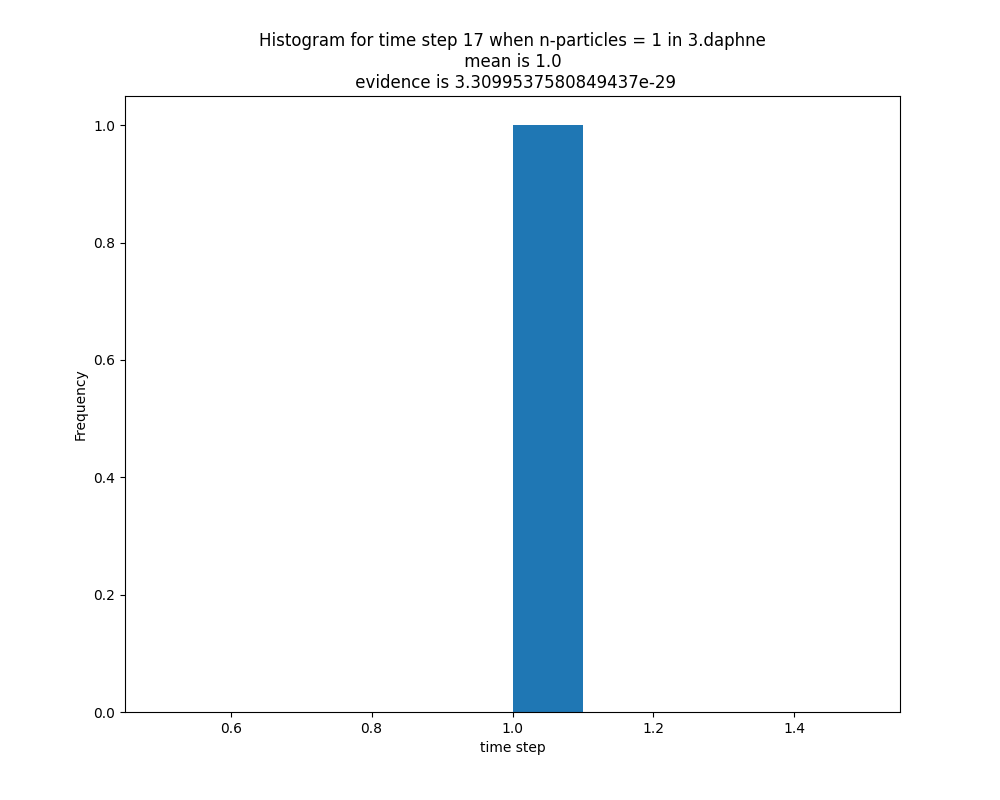
\includegraphics[width=0.3\textwidth]{../figs/3_daphne_1_17}%
        \label{fig:b}%
        }%
\end{figure}

\newpage
\item n-particles = 10

\begin{figure}[!htp]
	\centering
	 \subfloat[Samples from the posterior for time step]{%
        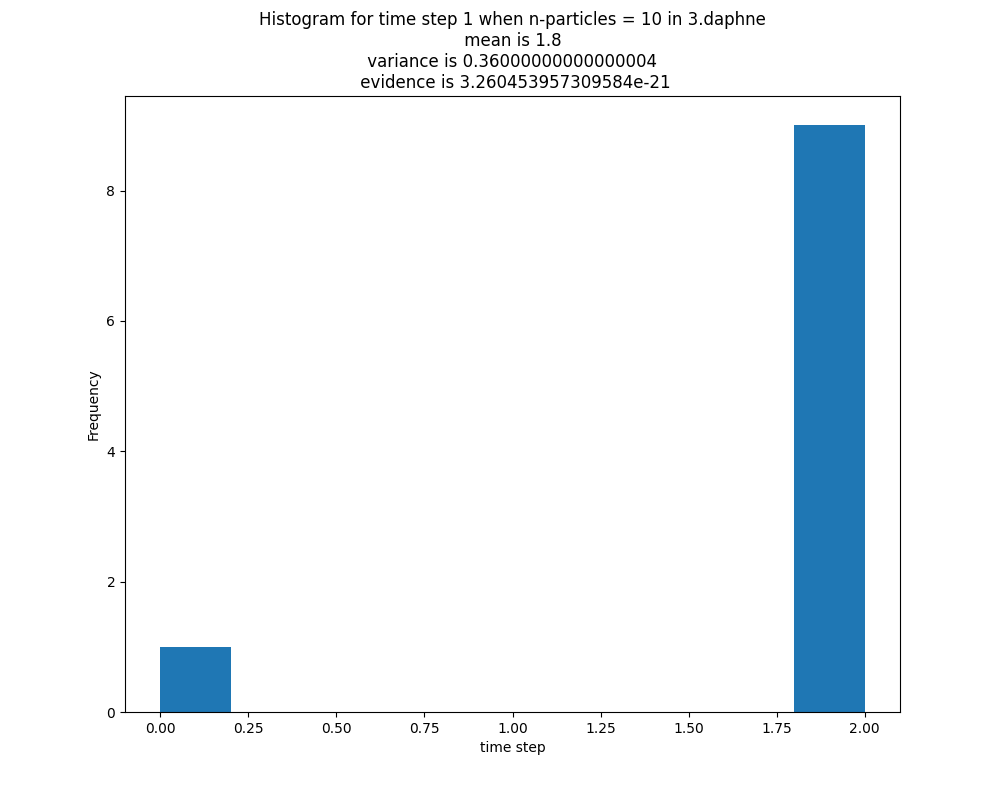
\includegraphics[width=0.3\textwidth]{../figs/3_daphne_10_1}%
        \label{fig:a}%
        }%
    \hfill%
    \subfloat[Samples from the posterior for time step]{%
        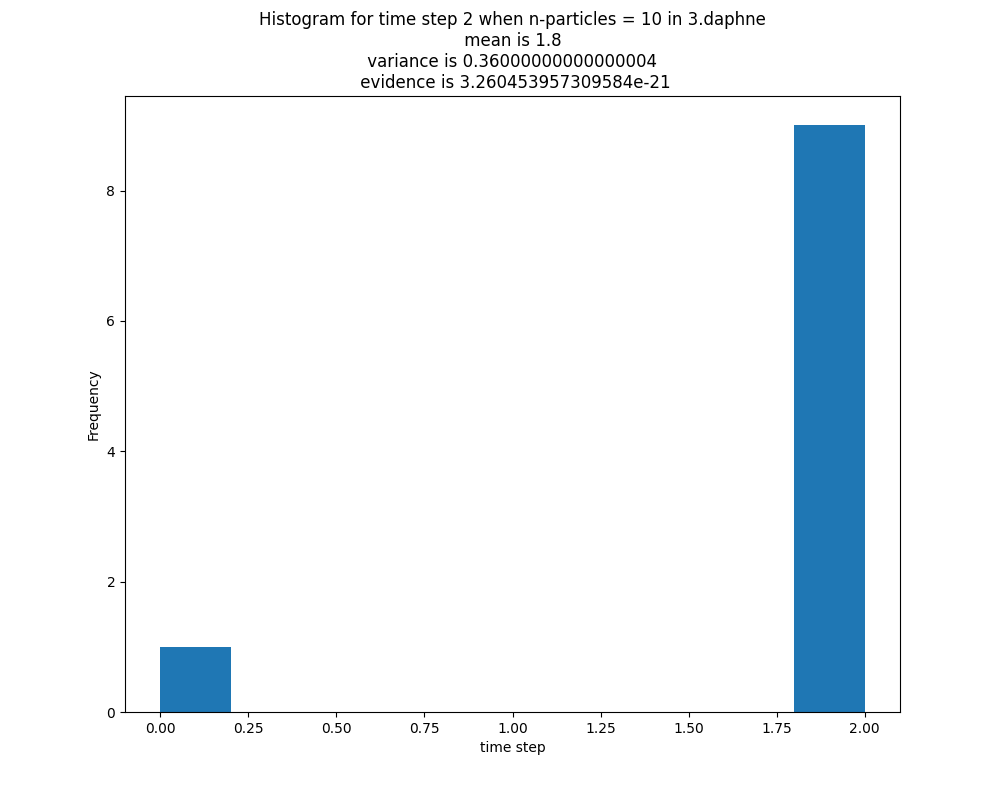
\includegraphics[width=0.3\textwidth]{../figs/3_daphne_10_2}%
        \label{fig:b}%
        }%
  \hfill
   \subfloat[Samples from the posterior for time step]{%
   	  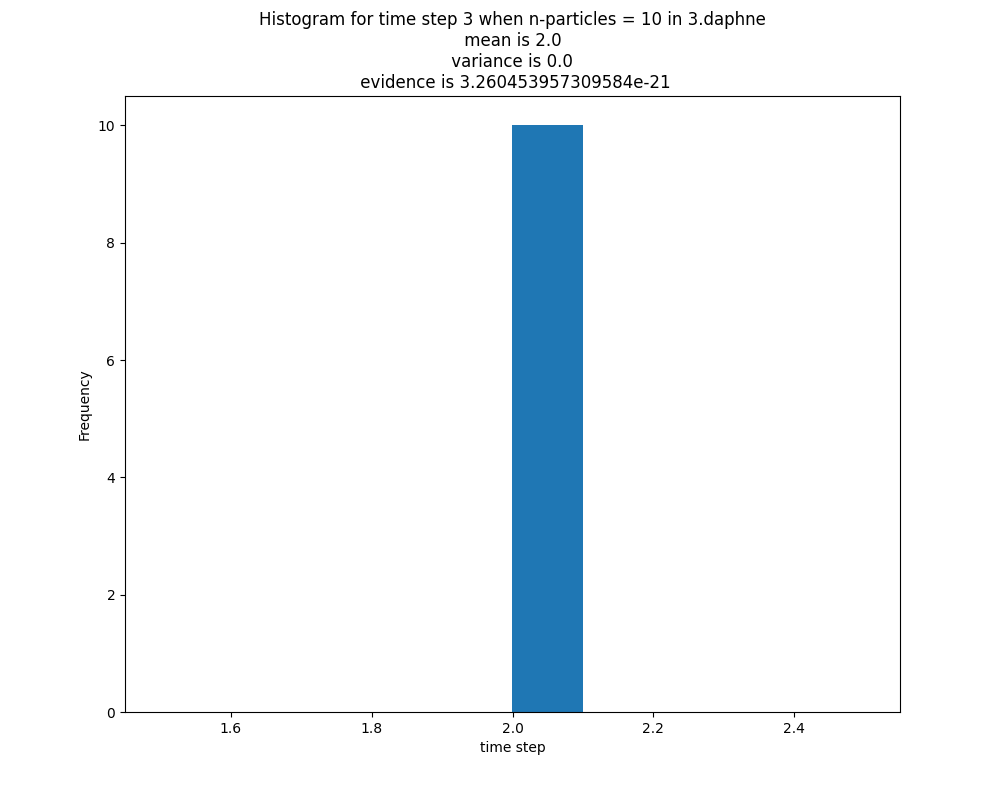
\includegraphics[width=0.3\textwidth]{../figs/3_daphne_10_3}%
   	  \label{fig:a}%
   	  }%
   	  
   \centering
	 \subfloat[Samples from the posterior for time step]{%
        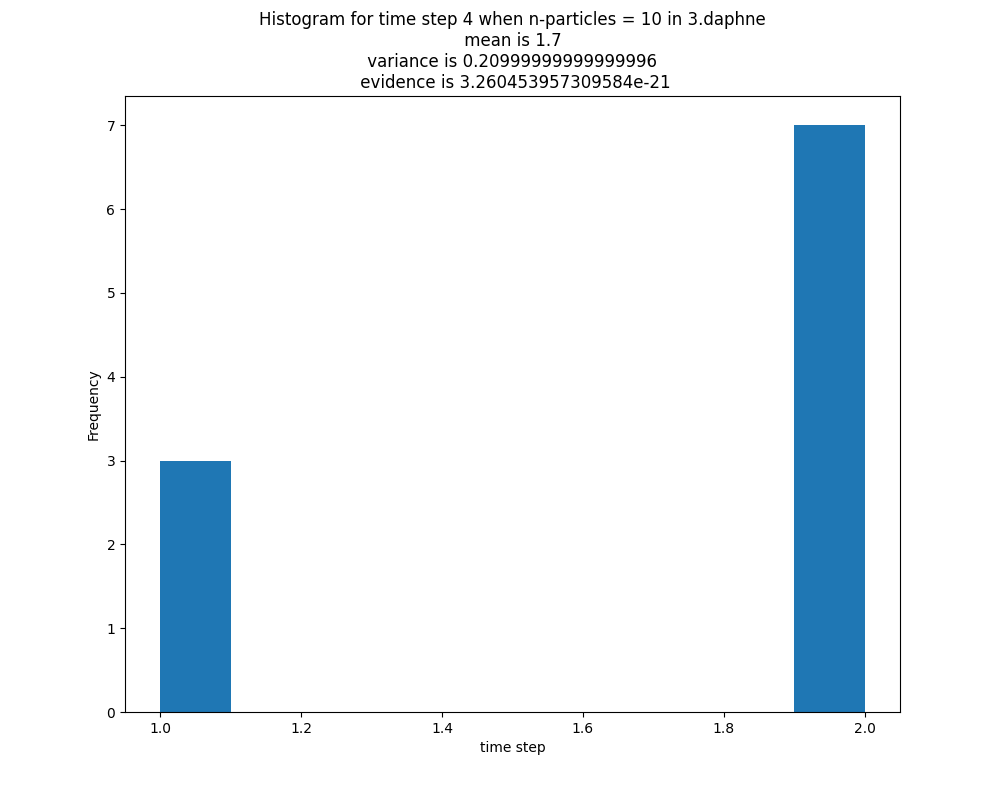
\includegraphics[width=0.3\textwidth]{../figs/3_daphne_10_4}%
        \label{fig:d}%
        }%       
	\hfill
	 \subfloat[Samples from the posterior for time step]{%
        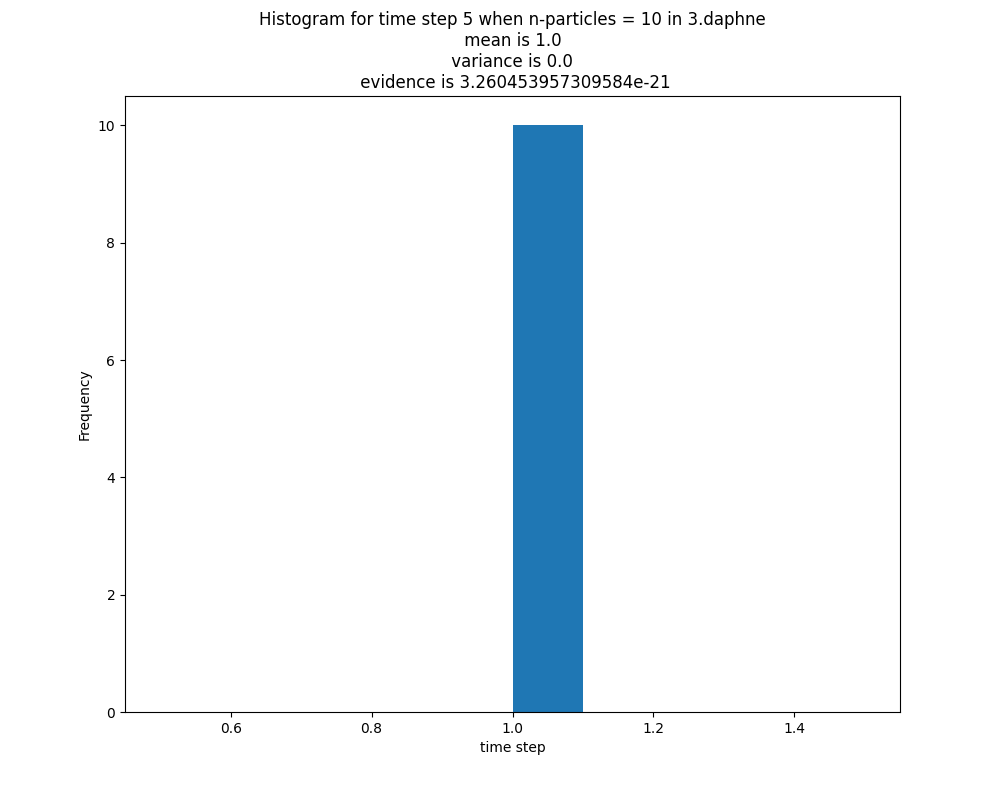
\includegraphics[width=0.3\textwidth]{../figs/3_daphne_10_5}%
        \label{fig:a}%
        }%
    \hfill%
    \subfloat[Samples from the posterior for time step]{%
        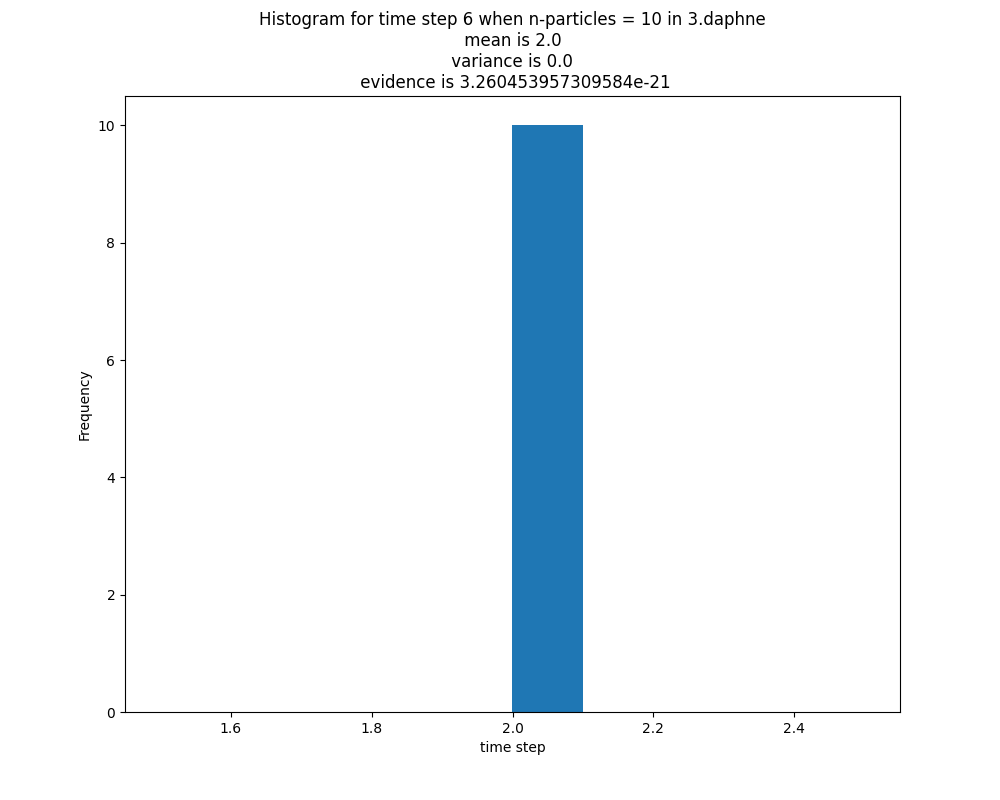
\includegraphics[width=0.3\textwidth]{../figs/3_daphne_10_6}%
        \label{fig:b}%
        }%
        
   \centering
	 \subfloat[Samples from the posterior for time step]{%
        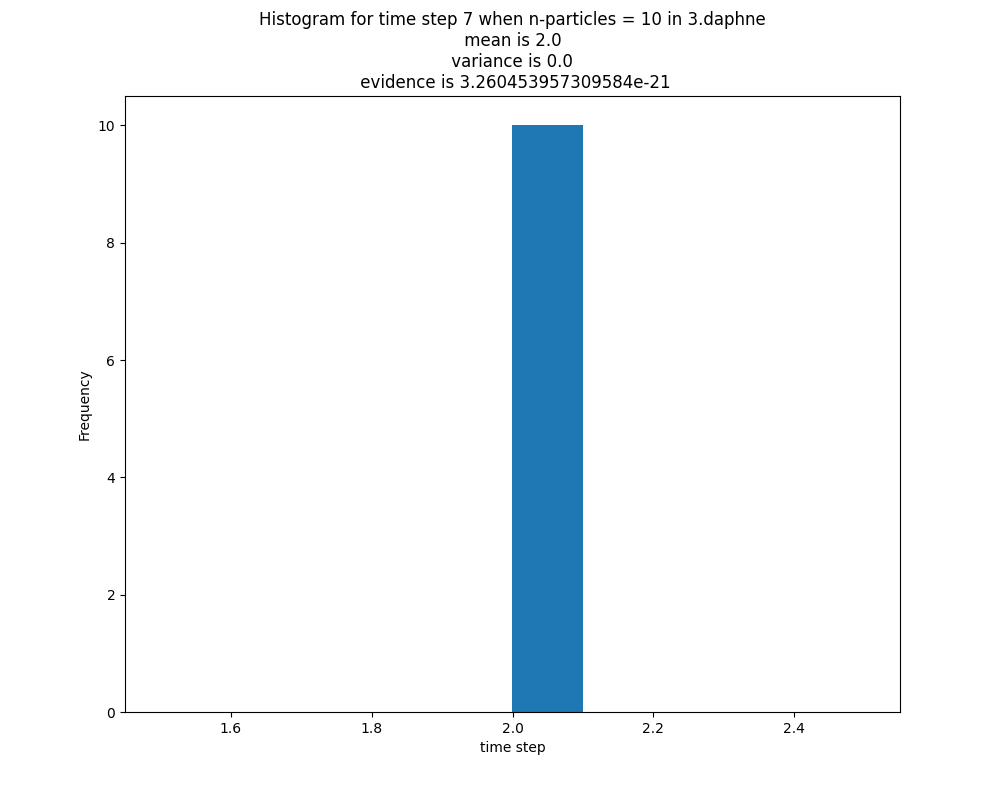
\includegraphics[width=0.3\textwidth]{../figs/3_daphne_10_7}%
        \label{fig:a}%
        }%
    \hfill%
    \subfloat[Samples from the posterior for time step]{%
        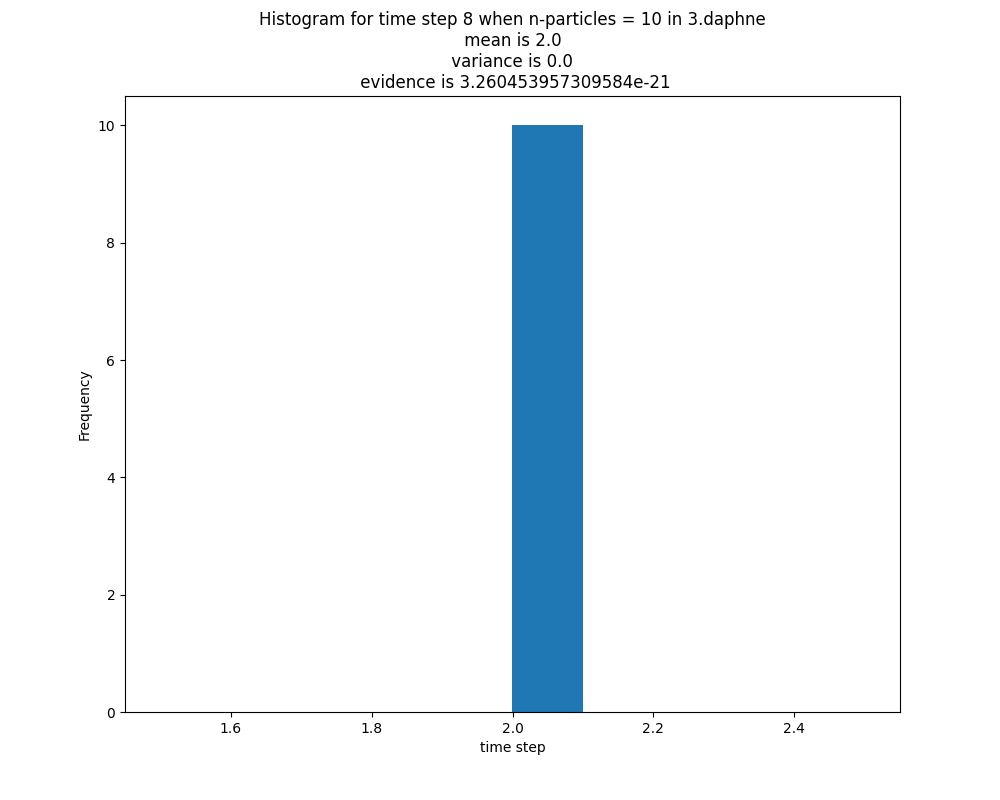
\includegraphics[width=0.3\textwidth]{../figs/3_daphne_10_8}%
        \label{fig:b}%
        }%
  \hfill
   \subfloat[Samples from the posterior for time step]{%
   	  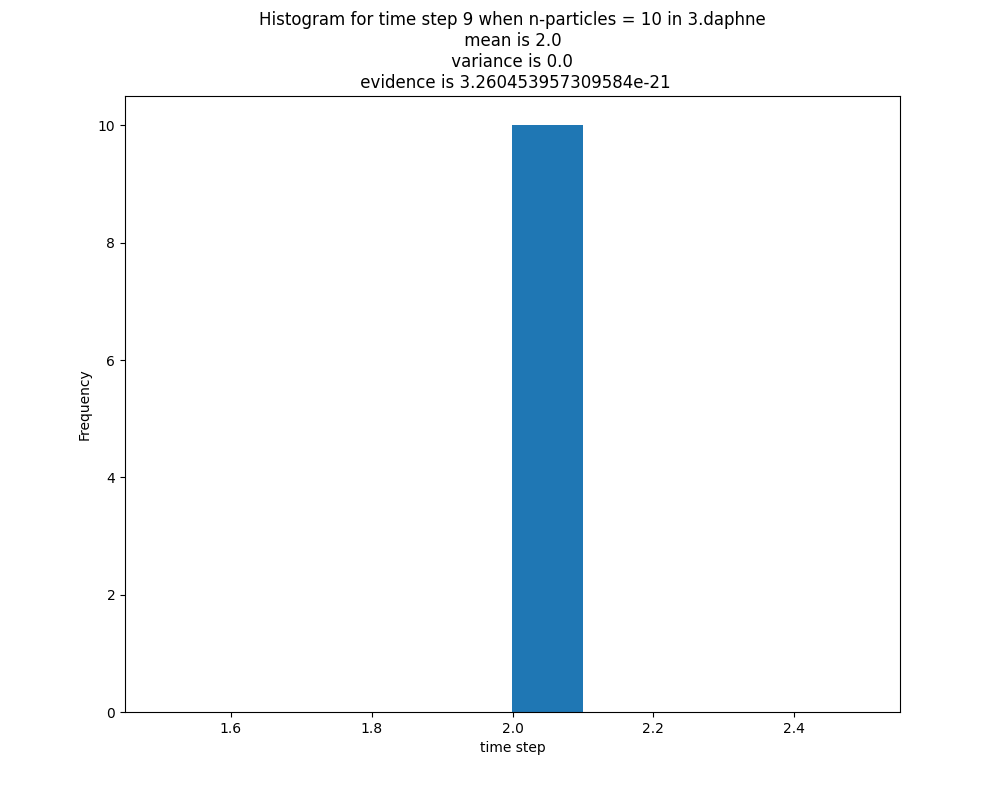
\includegraphics[width=0.3\textwidth]{../figs/3_daphne_10_9}%
   	  \label{fig:a}%
   	  }%
   	  
   \centering
	 \subfloat[Samples from the posterior for time step]{%
        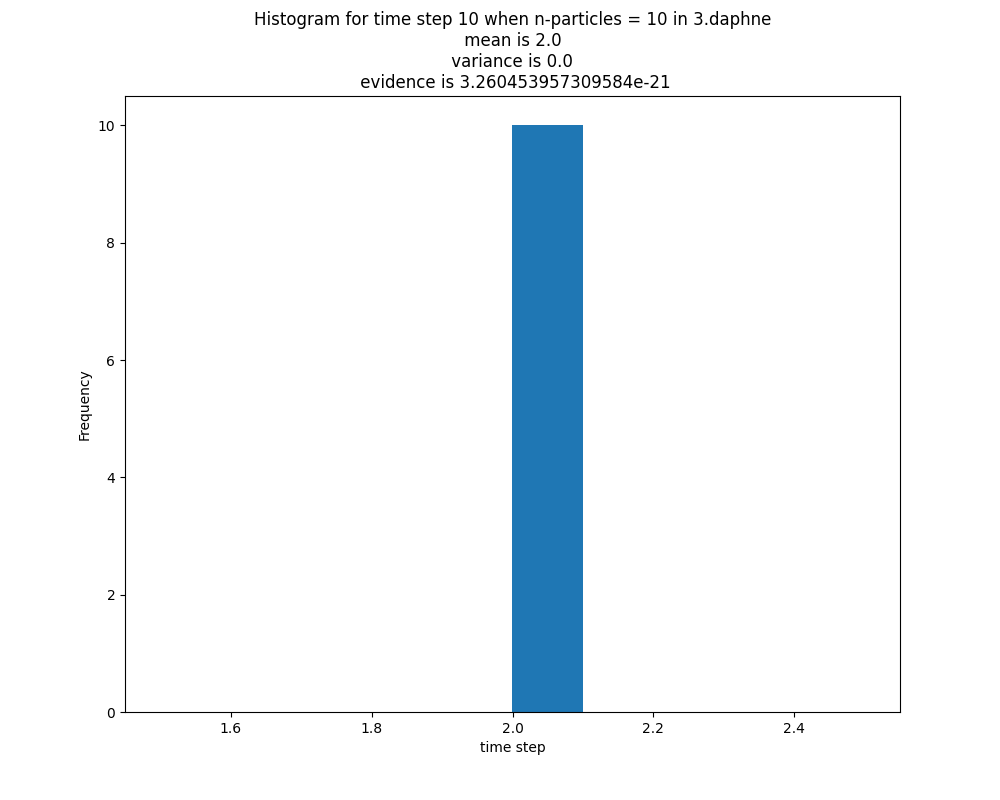
\includegraphics[width=0.3\textwidth]{../figs/3_daphne_10_10}%
        \label{fig:d}%
        }%       
	\hfill
	 \subfloat[Samples from the posterior for time step]{%
        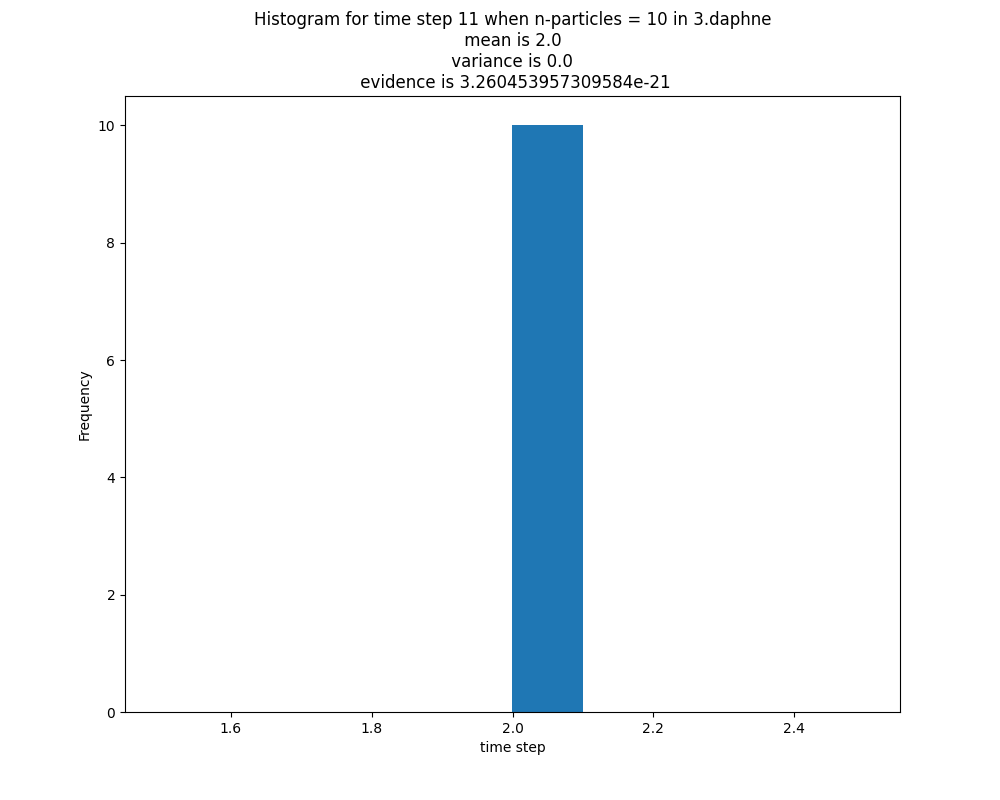
\includegraphics[width=0.3\textwidth]{../figs/3_daphne_10_11}%
        \label{fig:a}%
        }%
    \hfill%
    \subfloat[Samples from the posterior for time step]{%
        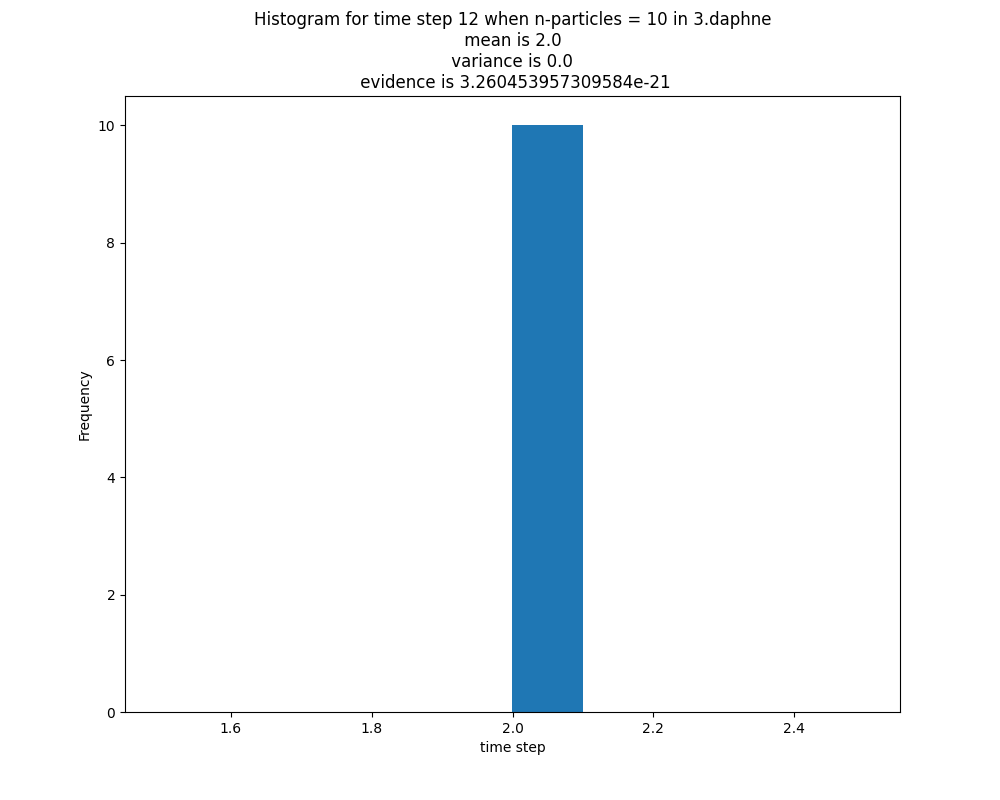
\includegraphics[width=0.3\textwidth]{../figs/3_daphne_10_12}%
        \label{fig:b}%
        }%
\end{figure}

\begin{figure}[!htp]
	\centering
	 \subfloat[Samples from the posterior for time step]{%
        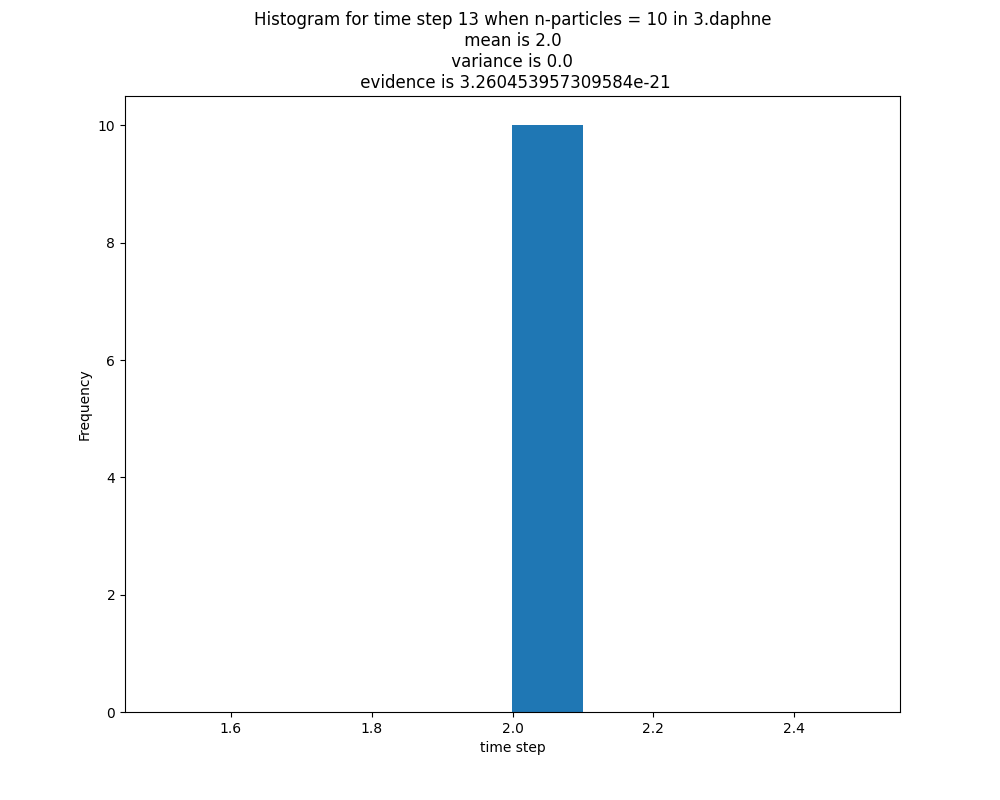
\includegraphics[width=0.3\textwidth]{../figs/3_daphne_10_13}%
        \label{fig:a}%
        }%
    \hfill%
    \subfloat[Samples from the posterior for time step]{%
        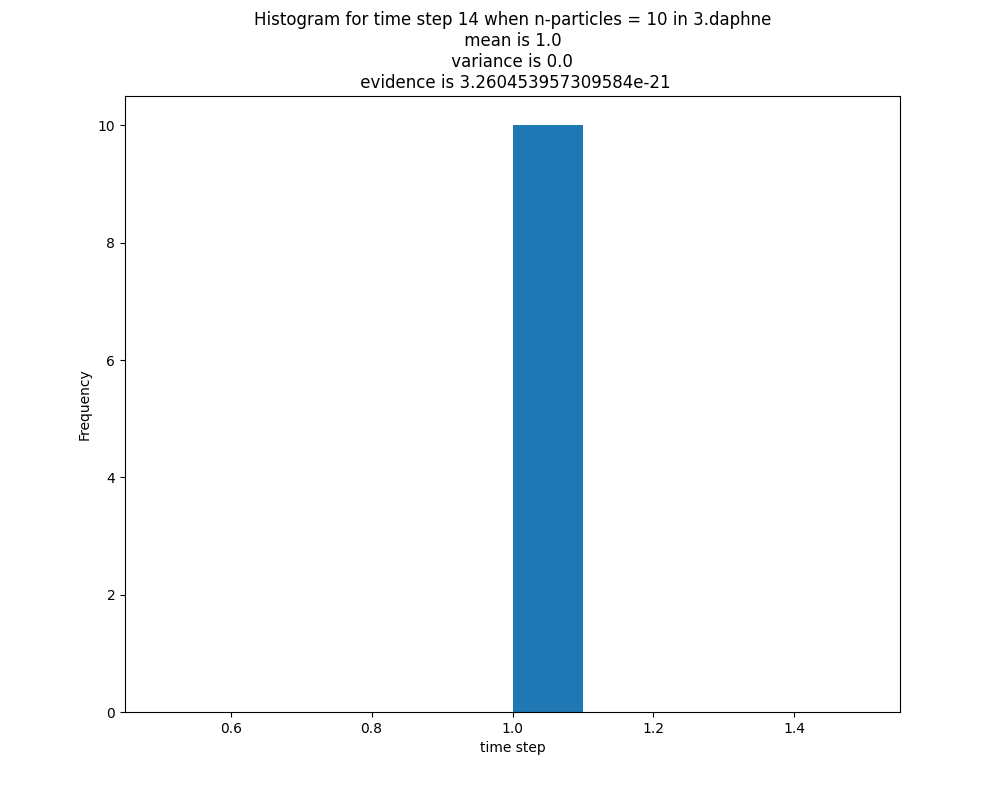
\includegraphics[width=0.3\textwidth]{../figs/3_daphne_10_14}%
        \label{fig:b}%
        }%
  \hfill
   \subfloat[Samples from the posterior for time step]{%
   	  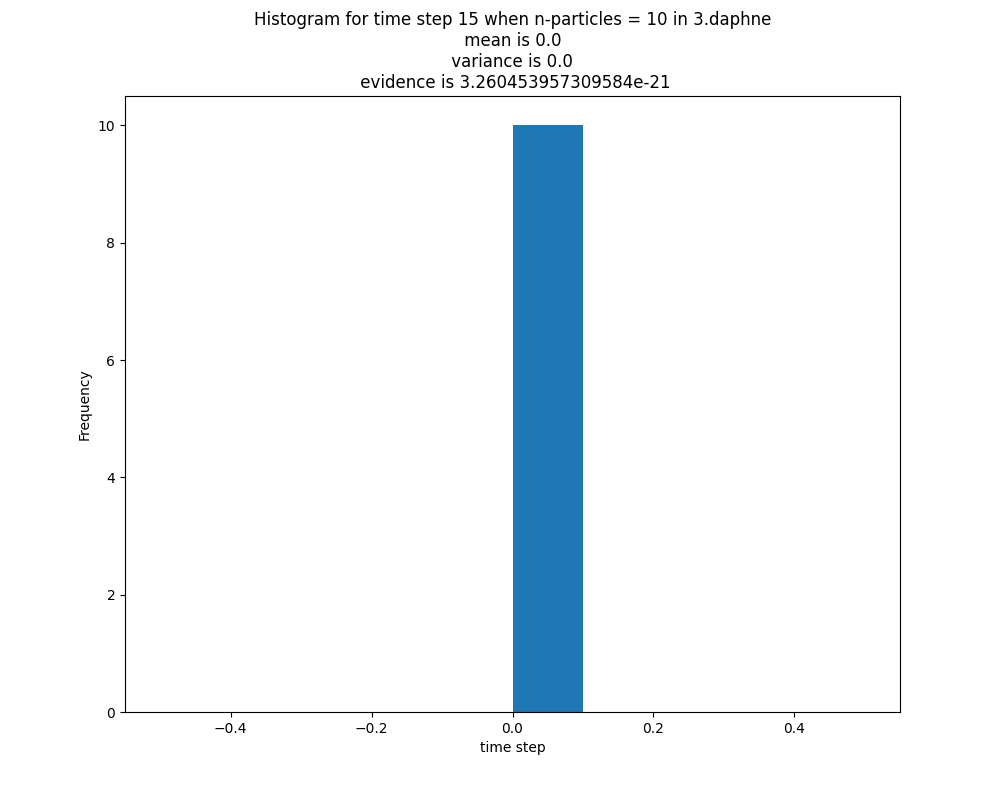
\includegraphics[width=0.3\textwidth]{../figs/3_daphne_10_15}%
   	  \label{fig:a}%
   	  }%
   	  
   \centering
	 \subfloat[Samples from the posterior for time step]{%
        \includegraphics[width=0.3\textwidth]{../figs/3_daphne_10_16}%
        \label{fig:a}%
        }%
    \hfill%
    \subfloat[Samples from the posterior for time step]{%
        \includegraphics[width=0.3\textwidth]{../figs/3_daphne_10_17}%
        \label{fig:b}%
        }%
\end{figure}

\newpage n-particles = 100

\begin{figure}[!htp]
	\centering
	 \subfloat[Samples from the posterior for time step]{%
        \includegraphics[width=0.3\textwidth]{../figs/3_daphne_100_1}%
        \label{fig:a}%
        }%
    \hfill%
    \subfloat[Samples from the posterior for time step]{%
        \includegraphics[width=0.3\textwidth]{../figs/3_daphne_100_2}%
        \label{fig:b}%
        }%
  \hfill
   \subfloat[Samples from the posterior for time step]{%
   	  \includegraphics[width=0.3\textwidth]{../figs/3_daphne_100_3}%
   	  \label{fig:a}%
   	  }%
   	  
   \centering
	 \subfloat[Samples from the posterior for time step]{%
        \includegraphics[width=0.3\textwidth]{../figs/3_daphne_100_4}%
        \label{fig:d}%
        }%       
	\hfill
	 \subfloat[Samples from the posterior for time step]{%
        \includegraphics[width=0.3\textwidth]{../figs/3_daphne_100_5}%
        \label{fig:a}%
        }%
    \hfill%
    \subfloat[Samples from the posterior for time step]{%
        \includegraphics[width=0.3\textwidth]{../figs/3_daphne_100_6}%
        \label{fig:b}%
        }%
        
   \centering
	 \subfloat[Samples from the posterior for time step]{%
        \includegraphics[width=0.3\textwidth]{../figs/3_daphne_100_7}%
        \label{fig:a}%
        }%
    \hfill%
    \subfloat[Samples from the posterior for time step]{%
        \includegraphics[width=0.3\textwidth]{../figs/3_daphne_100_8}%
        \label{fig:b}%
        }%
  \hfill
   \subfloat[Samples from the posterior for time step]{%
   	  \includegraphics[width=0.3\textwidth]{../figs/3_daphne_100_9}%
   	  \label{fig:a}%
   	  }%
   	  
   \centering
	 \subfloat[Samples from the posterior for time step]{%
        \includegraphics[width=0.3\textwidth]{../figs/3_daphne_100_10}%
        \label{fig:d}%
        }%       
	\hfill
	 \subfloat[Samples from the posterior for time step]{%
        \includegraphics[width=0.3\textwidth]{../figs/3_daphne_100_11}%
        \label{fig:a}%
        }%
    \hfill%
    \subfloat[Samples from the posterior for time step]{%
        \includegraphics[width=0.3\textwidth]{../figs/3_daphne_100_12}%
        \label{fig:b}%
        }%
\end{figure}

\begin{figure}[!htp]
	\centering
	 \subfloat[Samples from the posterior for time step]{%
        \includegraphics[width=0.3\textwidth]{../figs/3_daphne_100_13}%
        \label{fig:a}%
        }%
    \hfill%
    \subfloat[Samples from the posterior for time step]{%
        \includegraphics[width=0.3\textwidth]{../figs/3_daphne_100_14}%
        \label{fig:b}%
        }%
  \hfill
   \subfloat[Samples from the posterior for time step]{%
   	  \includegraphics[width=0.3\textwidth]{../figs/3_daphne_100_15}%
   	  \label{fig:a}%
   	  }%
   	  
   \centering
	 \subfloat[Samples from the posterior for time step]{%
        \includegraphics[width=0.3\textwidth]{../figs/3_daphne_100_16}%
        \label{fig:a}%
        }%
    \hfill%
    \subfloat[Samples from the posterior for time step]{%
        \includegraphics[width=0.3\textwidth]{../figs/3_daphne_100_17}%
        \label{fig:b}%
        }%
\end{figure}

\newpage
\item n-particles = 1000
\begin{figure}[!htp]
	\centering
	 \subfloat[Samples from the posterior for time step]{%
        \includegraphics[width=0.3\textwidth]{../figs/3_daphne_1000_1}%
        \label{fig:a}%
        }%
    \hfill%
    \subfloat[Samples from the posterior for time step]{%
        \includegraphics[width=0.3\textwidth]{../figs/3_daphne_1000_2}%
        \label{fig:b}%
        }%
  \hfill
   \subfloat[Samples from the posterior for time step]{%
   	  \includegraphics[width=0.3\textwidth]{../figs/3_daphne_1000_3}%
   	  \label{fig:a}%
   	  }%
   	  
   \centering
	 \subfloat[Samples from the posterior for time step]{%
        \includegraphics[width=0.3\textwidth]{../figs/3_daphne_1000_4}%
        \label{fig:d}%
        }%       
	\hfill
	 \subfloat[Samples from the posterior for time step]{%
        \includegraphics[width=0.3\textwidth]{../figs/3_daphne_1000_5}%
        \label{fig:a}%
        }%
    \hfill%
    \subfloat[Samples from the posterior for time step]{%
        \includegraphics[width=0.3\textwidth]{../figs/3_daphne_1000_6}%
        \label{fig:b}%
        }%
        
   \centering
	 \subfloat[Samples from the posterior for time step]{%
        \includegraphics[width=0.3\textwidth]{../figs/3_daphne_1000_7}%
        \label{fig:a}%
        }%
    \hfill%
    \subfloat[Samples from the posterior for time step]{%
        \includegraphics[width=0.3\textwidth]{../figs/3_daphne_1000_8}%
        \label{fig:b}%
        }%
  \hfill
   \subfloat[Samples from the posterior for time step]{%
   	  \includegraphics[width=0.3\textwidth]{../figs/3_daphne_1000_9}%
   	  \label{fig:a}%
   	  }%
   	  
   \centering
	 \subfloat[Samples from the posterior for time step]{%
        \includegraphics[width=0.3\textwidth]{../figs/3_daphne_1000_10}%
        \label{fig:d}%
        }%       
	\hfill
	 \subfloat[Samples from the posterior for time step]{%
        \includegraphics[width=0.3\textwidth]{../figs/3_daphne_1000_11}%
        \label{fig:a}%
        }%
    \hfill%
    \subfloat[Samples from the posterior for time step]{%
        \includegraphics[width=0.3\textwidth]{../figs/3_daphne_1000_12}%
        \label{fig:b}%
        }%
\end{figure}

\begin{figure}[!htp]
	\centering
	 \subfloat[Samples from the posterior for time step]{%
        \includegraphics[width=0.3\textwidth]{../figs/3_daphne_1000_13}%
        \label{fig:a}%
        }%
    \hfill%
    \subfloat[Samples from the posterior for time step]{%
        \includegraphics[width=0.3\textwidth]{../figs/3_daphne_1000_14}%
        \label{fig:b}%
        }%
  \hfill
   \subfloat[Samples from the posterior for time step]{%
   	  \includegraphics[width=0.3\textwidth]{../figs/3_daphne_1000_15}%
   	  \label{fig:a}%
   	  }%
   	  
   \centering
	 \subfloat[Samples from the posterior for time step]{%
        \includegraphics[width=0.3\textwidth]{../figs/3_daphne_1000_16}%
        \label{fig:a}%
        }%
    \hfill%
    \subfloat[Samples from the posterior for time step]{%
        \includegraphics[width=0.3\textwidth]{../figs/3_daphne_1000_17}%
        \label{fig:b}%
        }%
\end{figure}

\newpage
\item n-particles = 10000

\begin{figure}[!htp]
	\centering
	 \subfloat[Samples from the posterior for time step]{%
        \includegraphics[width=0.3\textwidth]{../figs/3_daphne_10000_1}%
        \label{fig:a}%
        }%
    \hfill%
    \subfloat[Samples from the posterior for time step]{%
        \includegraphics[width=0.3\textwidth]{../figs/3_daphne_10000_2}%
        \label{fig:b}%
        }%
  \hfill
   \subfloat[Samples from the posterior for time step]{%
   	  \includegraphics[width=0.3\textwidth]{../figs/3_daphne_10000_3}%
   	  \label{fig:a}%
   	  }%
   	  
   \centering
	 \subfloat[Samples from the posterior for time step]{%
        \includegraphics[width=0.3\textwidth]{../figs/3_daphne_10000_4}%
        \label{fig:d}%
        }%       
	\hfill
	 \subfloat[Samples from the posterior for time step]{%
        \includegraphics[width=0.3\textwidth]{../figs/3_daphne_10000_5}%
        \label{fig:a}%
        }%
    \hfill%
    \subfloat[Samples from the posterior for time step]{%
        \includegraphics[width=0.3\textwidth]{../figs/3_daphne_10000_6}%
        \label{fig:b}%
        }%
        
   \centering
	 \subfloat[Samples from the posterior for time step]{%
        \includegraphics[width=0.3\textwidth]{../figs/3_daphne_10000_7}%
        \label{fig:a}%
        }%
    \hfill%
    \subfloat[Samples from the posterior for time step]{%
        \includegraphics[width=0.3\textwidth]{../figs/3_daphne_10000_8}%
        \label{fig:b}%
        }%
  \hfill
   \subfloat[Samples from the posterior for time step]{%
   	  \includegraphics[width=0.3\textwidth]{../figs/3_daphne_10000_9}%
   	  \label{fig:a}%
   	  }%
   	  
   \centering
	 \subfloat[Samples from the posterior for time step]{%
        \includegraphics[width=0.3\textwidth]{../figs/3_daphne_10000_10}%
        \label{fig:d}%
        }%       
	\hfill
	 \subfloat[Samples from the posterior for time step]{%
        \includegraphics[width=0.3\textwidth]{../figs/3_daphne_10000_11}%
        \label{fig:a}%
        }%
    \hfill%
    \subfloat[Samples from the posterior for time step]{%
        \includegraphics[width=0.3\textwidth]{../figs/3_daphne_10000_12}%
        \label{fig:b}%
        }%
\end{figure}

\begin{figure}[!htp]
	\centering
	 \subfloat[Samples from the posterior for time step]{%
        \includegraphics[width=0.3\textwidth]{../figs/3_daphne_10000_13}%
        \label{fig:a}%
        }%
    \hfill%
    \subfloat[Samples from the posterior for time step]{%
        \includegraphics[width=0.3\textwidth]{../figs/3_daphne_10000_14}%
        \label{fig:b}%
        }%
  \hfill
   \subfloat[Samples from the posterior for time step]{%
   	  \includegraphics[width=0.3\textwidth]{../figs/3_daphne_10000_15}%
   	  \label{fig:a}%
   	  }%
   	  
   \centering
	 \subfloat[Samples from the posterior for time step]{%
        \includegraphics[width=0.3\textwidth]{../figs/3_daphne_10000_16}%
        \label{fig:a}%
        }%
    \hfill%
    \subfloat[Samples from the posterior for time step]{%
        \includegraphics[width=0.3\textwidth]{../figs/3_daphne_10000_17}%
        \label{fig:b}%
        }%
\end{figure}

\newpage
\item n-particles = 10000
\begin{figure}[!htp]
	\centering
	 \subfloat[Samples from the posterior for time step]{%
        \includegraphics[width=0.3\textwidth]{../figs/3_daphne_10000_1}%
        \label{fig:a}%
        }%
    \hfill%
    \subfloat[Samples from the posterior for time step]{%
        \includegraphics[width=0.3\textwidth]{../figs/3_daphne_10000_2}%
        \label{fig:b}%
        }%
  \hfill
   \subfloat[Samples from the posterior for time step]{%
   	  \includegraphics[width=0.3\textwidth]{../figs/3_daphne_10000_3}%
   	  \label{fig:a}%
   	  }%
   	  
   \centering
	 \subfloat[Samples from the posterior for time step]{%
        \includegraphics[width=0.3\textwidth]{../figs/3_daphne_10000_4}%
        \label{fig:d}%
        }%       
	\hfill
	 \subfloat[Samples from the posterior for time step]{%
        \includegraphics[width=0.3\textwidth]{../figs/3_daphne_10000_5}%
        \label{fig:a}%
        }%
    \hfill%
    \subfloat[Samples from the posterior for time step]{%
        \includegraphics[width=0.3\textwidth]{../figs/3_daphne_10000_6}%
        \label{fig:b}%
        }%
        
   \centering
	 \subfloat[Samples from the posterior for time step]{%
        \includegraphics[width=0.3\textwidth]{../figs/3_daphne_10000_7}%
        \label{fig:a}%
        }%
    \hfill%
    \subfloat[Samples from the posterior for time step]{%
        \includegraphics[width=0.3\textwidth]{../figs/3_daphne_10000_8}%
        \label{fig:b}%
        }%
  \hfill
   \subfloat[Samples from the posterior for time step]{%
   	  \includegraphics[width=0.3\textwidth]{../figs/3_daphne_10000_9}%
   	  \label{fig:a}%
   	  }%
   	  
   \centering
	 \subfloat[Samples from the posterior for time step]{%
        \includegraphics[width=0.3\textwidth]{../figs/3_daphne_10000_10}%
        \label{fig:d}%
        }%       
	\hfill
	 \subfloat[Samples from the posterior for time step]{%
        \includegraphics[width=0.3\textwidth]{../figs/3_daphne_10000_11}%
        \label{fig:a}%
        }%
    \hfill%
    \subfloat[Samples from the posterior for time step]{%
        \includegraphics[width=0.3\textwidth]{../figs/3_daphne_10000_12}%
        \label{fig:b}%
        }%
\end{figure}

\begin{figure}[!htp]
	\centering
	 \subfloat[Samples from the posterior for time step]{%
        \includegraphics[width=0.3\textwidth]{../figs/3_daphne_10000_13}%
        \label{fig:a}%
        }%
    \hfill%
    \subfloat[Samples from the posterior for time step]{%
        \includegraphics[width=0.3\textwidth]{../figs/3_daphne_10000_14}%
        \label{fig:b}%
        }%
  \hfill
   \subfloat[Samples from the posterior for time step]{%
   	  \includegraphics[width=0.3\textwidth]{../figs/3_daphne_10000_15}%
   	  \label{fig:a}%
   	  }%
   	  
   \centering
	 \subfloat[Samples from the posterior for time step]{%
        \includegraphics[width=0.3\textwidth]{../figs/3_daphne_10000_16}%
        \label{fig:a}%
        }%
    \hfill%
    \subfloat[Samples from the posterior for time step]{%
        \includegraphics[width=0.3\textwidth]{../figs/3_daphne_10000_17}%
        \label{fig:b}%
        }%
\end{figure}

\newpage
\item n-particles = 100000
\begin{figure}[!htp]
	\centering
	 \subfloat[Samples from the posterior for time step]{%
        \includegraphics[width=0.3\textwidth]{../figs/3_daphne_100000_1}%
        \label{fig:a}%
        }%
    \hfill%
    \subfloat[Samples from the posterior for time step]{%
        \includegraphics[width=0.3\textwidth]{../figs/3_daphne_100000_2}%
        \label{fig:b}%
        }%
  \hfill
   \subfloat[Samples from the posterior for time step]{%
   	  \includegraphics[width=0.3\textwidth]{../figs/3_daphne_100000_3}%
   	  \label{fig:a}%
   	  }%
   	  
   \centering
	 \subfloat[Samples from the posterior for time step]{%
        \includegraphics[width=0.3\textwidth]{../figs/3_daphne_100000_4}%
        \label{fig:d}%
        }%       
	\hfill
	 \subfloat[Samples from the posterior for time step]{%
        \includegraphics[width=0.3\textwidth]{../figs/3_daphne_100000_5}%
        \label{fig:a}%
        }%
    \hfill%
    \subfloat[Samples from the posterior for time step]{%
        \includegraphics[width=0.3\textwidth]{../figs/3_daphne_100000_6}%
        \label{fig:b}%
        }%
        
   \centering
	 \subfloat[Samples from the posterior for time step]{%
        \includegraphics[width=0.3\textwidth]{../figs/3_daphne_100000_7}%
        \label{fig:a}%
        }%
    \hfill%
    \subfloat[Samples from the posterior for time step]{%
        \includegraphics[width=0.3\textwidth]{../figs/3_daphne_100000_8}%
        \label{fig:b}%
        }%
  \hfill
   \subfloat[Samples from the posterior for time step]{%
   	  \includegraphics[width=0.3\textwidth]{../figs/3_daphne_100000_9}%
   	  \label{fig:a}%
   	  }%
   	  
   \centering
	 \subfloat[Samples from the posterior for time step]{%
        \includegraphics[width=0.3\textwidth]{../figs/3_daphne_100000_10}%
        \label{fig:d}%
        }%       
	\hfill
	 \subfloat[Samples from the posterior for time step]{%
        \includegraphics[width=0.3\textwidth]{../figs/3_daphne_100000_11}%
        \label{fig:a}%
        }%
    \hfill%
    \subfloat[Samples from the posterior for time step]{%
        \includegraphics[width=0.3\textwidth]{../figs/3_daphne_100000_12}%
        \label{fig:b}%
        }%
\end{figure}

\begin{figure}[!htp]
	\centering
	 \subfloat[Samples from the posterior for time step]{%
        \includegraphics[width=0.3\textwidth]{../figs/3_daphne_100000_13}%
        \label{fig:a}%
        }%
    \hfill%
    \subfloat[Samples from the posterior for time step]{%
        \includegraphics[width=0.3\textwidth]{../figs/3_daphne_100000_14}%
        \label{fig:b}%
        }%
  \hfill
   \subfloat[Samples from the posterior for time step]{%
   	  \includegraphics[width=0.3\textwidth]{../figs/3_daphne_100000_15}%
   	  \label{fig:a}%
   	  }%
   	  
   \centering
	 \subfloat[Samples from the posterior for time step]{%
        \includegraphics[width=0.3\textwidth]{../figs/3_daphne_100000_16}%
        \label{fig:a}%
        }%
    \hfill%
    \subfloat[Samples from the posterior for time step]{%
        \includegraphics[width=0.3\textwidth]{../figs/3_daphne_100000_17}%
        \label{fig:b}%
        }%
\end{figure}
\end{itemize}

\begin{figure}[!ht]
	\centering
	\includegraphics[scale=0.5]{../figs/3_daphne_evidence}
\end{figure}

\newpage
\item Program 4
\begin{figure}[!htp]
	\centering
	 \subfloat[Samples from the posterior for mu]{%
        \includegraphics[width=0.5\textwidth]{../figs/4_daphne_1}%
        \label{fig:a}%
        }%
    \hfill%
    \subfloat[Samples from the posterior for mu]{%
        \includegraphics[width=0.5\textwidth]{../figs/4_daphne_10}%
        \label{fig:b}%
        }%
   \centering
   
   \subfloat[Samples from the posterior for mu]{%
   	  \includegraphics[width=0.5\textwidth]{../figs/4_daphne_100}%
   	  \label{fig:a}%
   	  }%
   \hfill%
	 \subfloat[Samples from the posterior for mu]{%
        \includegraphics[width=0.5\textwidth]{../figs/4_daphne_1000}%
        \label{fig:d}%
        }%

	\centering
	 \subfloat[Samples from the posterior for mu]{%
        \includegraphics[width=0.5\textwidth]{../figs/4_daphne_10000}%
        \label{fig:a}%
        }%
    \hfill%
    \subfloat[Samples from the posterior for mu]{%
        \includegraphics[width=0.5\textwidth]{../figs/4_daphne_100000}%
        \label{fig:b}%
        }%
\end{figure}

\begin{figure}[!ht]
	\centering
	\includegraphics[scale=0.5]{../figs/4_daphne_trace_plot}
	\includegraphics[scale=0.5]{../figs/4_daphne_evidence}
\end{figure}

\end{enumerate}
\end{document}